\documentclass[12pt,landscape]{article}

%\usepackage{lmodern}
\usepackage{amssymb,amsmath}
\usepackage{bm}
\usepackage{graphicx}
\usepackage{microtype}
\usepackage{hyperref}
\pagestyle{empty}
\usepackage{titlesec}
\titleformat*{\section}{\LARGE\bfseries}
\titleformat*{\subsection}{\LARGE\bfseries}
\titleformat*{\subsubsection}{\LARGE\bfseries}
\setlength{\parindent}{0pt}
\setlength{\parskip}{1.2ex}
\setlength{\parindent}{0pt}
\setlength{\parskip}{1.2ex}

\setlength{\oddsidemargin}{-16mm}
\setlength{\textwidth}{260mm}
\setlength{\columnsep}{0.5in}
\setlength{\columnseprule}{1pt}
\setlength{\textheight}{202mm}
\setlength{\topmargin}{-32mm}
\setlength{\headsep}{0.25in}

\hypersetup
       {   pdfauthor = { Marco Fasondini },
           pdftitle={ foo },
           colorlinks=TRUE,
           linkcolor=black,
           citecolor=blue,
           urlcolor=blue
       }




\usepackage{upquote}
\usepackage{listings}
\usepackage{xcolor}
\lstset{
    basicstyle=\ttfamily\footnotesize,
    upquote=true,
    breaklines=true,
    breakindent=0pt,
    keepspaces=true,
    showspaces=false,
    columns=fullflexible,
    showtabs=false,
    showstringspaces=false,
    escapeinside={(*@}{@*)},
    extendedchars=true,
}
\newcommand{\HLJLt}[1]{#1}
\newcommand{\HLJLw}[1]{#1}
\newcommand{\HLJLe}[1]{#1}
\newcommand{\HLJLeB}[1]{#1}
\newcommand{\HLJLo}[1]{#1}
\newcommand{\HLJLk}[1]{\textcolor[RGB]{148,91,176}{\textbf{#1}}}
\newcommand{\HLJLkc}[1]{\textcolor[RGB]{59,151,46}{\textit{#1}}}
\newcommand{\HLJLkd}[1]{\textcolor[RGB]{214,102,97}{\textit{#1}}}
\newcommand{\HLJLkn}[1]{\textcolor[RGB]{148,91,176}{\textbf{#1}}}
\newcommand{\HLJLkp}[1]{\textcolor[RGB]{148,91,176}{\textbf{#1}}}
\newcommand{\HLJLkr}[1]{\textcolor[RGB]{148,91,176}{\textbf{#1}}}
\newcommand{\HLJLkt}[1]{\textcolor[RGB]{148,91,176}{\textbf{#1}}}
\newcommand{\HLJLn}[1]{#1}
\newcommand{\HLJLna}[1]{#1}
\newcommand{\HLJLnb}[1]{#1}
\newcommand{\HLJLnbp}[1]{#1}
\newcommand{\HLJLnc}[1]{#1}
\newcommand{\HLJLncB}[1]{#1}
\newcommand{\HLJLnd}[1]{\textcolor[RGB]{214,102,97}{#1}}
\newcommand{\HLJLne}[1]{#1}
\newcommand{\HLJLneB}[1]{#1}
\newcommand{\HLJLnf}[1]{\textcolor[RGB]{66,102,213}{#1}}
\newcommand{\HLJLnfm}[1]{\textcolor[RGB]{66,102,213}{#1}}
\newcommand{\HLJLnp}[1]{#1}
\newcommand{\HLJLnl}[1]{#1}
\newcommand{\HLJLnn}[1]{#1}
\newcommand{\HLJLno}[1]{#1}
\newcommand{\HLJLnt}[1]{#1}
\newcommand{\HLJLnv}[1]{#1}
\newcommand{\HLJLnvc}[1]{#1}
\newcommand{\HLJLnvg}[1]{#1}
\newcommand{\HLJLnvi}[1]{#1}
\newcommand{\HLJLnvm}[1]{#1}
\newcommand{\HLJLl}[1]{#1}
\newcommand{\HLJLld}[1]{\textcolor[RGB]{148,91,176}{\textit{#1}}}
\newcommand{\HLJLs}[1]{\textcolor[RGB]{201,61,57}{#1}}
\newcommand{\HLJLsa}[1]{\textcolor[RGB]{201,61,57}{#1}}
\newcommand{\HLJLsb}[1]{\textcolor[RGB]{201,61,57}{#1}}
\newcommand{\HLJLsc}[1]{\textcolor[RGB]{201,61,57}{#1}}
\newcommand{\HLJLsd}[1]{\textcolor[RGB]{201,61,57}{#1}}
\newcommand{\HLJLsdB}[1]{\textcolor[RGB]{201,61,57}{#1}}
\newcommand{\HLJLsdC}[1]{\textcolor[RGB]{201,61,57}{#1}}
\newcommand{\HLJLse}[1]{\textcolor[RGB]{59,151,46}{#1}}
\newcommand{\HLJLsh}[1]{\textcolor[RGB]{201,61,57}{#1}}
\newcommand{\HLJLsi}[1]{#1}
\newcommand{\HLJLso}[1]{\textcolor[RGB]{201,61,57}{#1}}
\newcommand{\HLJLsr}[1]{\textcolor[RGB]{201,61,57}{#1}}
\newcommand{\HLJLss}[1]{\textcolor[RGB]{201,61,57}{#1}}
\newcommand{\HLJLssB}[1]{\textcolor[RGB]{201,61,57}{#1}}
\newcommand{\HLJLnB}[1]{\textcolor[RGB]{59,151,46}{#1}}
\newcommand{\HLJLnbB}[1]{\textcolor[RGB]{59,151,46}{#1}}
\newcommand{\HLJLnfB}[1]{\textcolor[RGB]{59,151,46}{#1}}
\newcommand{\HLJLnh}[1]{\textcolor[RGB]{59,151,46}{#1}}
\newcommand{\HLJLni}[1]{\textcolor[RGB]{59,151,46}{#1}}
\newcommand{\HLJLnil}[1]{\textcolor[RGB]{59,151,46}{#1}}
\newcommand{\HLJLnoB}[1]{\textcolor[RGB]{59,151,46}{#1}}
\newcommand{\HLJLoB}[1]{\textcolor[RGB]{102,102,102}{\textbf{#1}}}
\newcommand{\HLJLow}[1]{\textcolor[RGB]{102,102,102}{\textbf{#1}}}
\newcommand{\HLJLp}[1]{#1}
\newcommand{\HLJLc}[1]{\textcolor[RGB]{153,153,119}{\textit{#1}}}
\newcommand{\HLJLch}[1]{\textcolor[RGB]{153,153,119}{\textit{#1}}}
\newcommand{\HLJLcm}[1]{\textcolor[RGB]{153,153,119}{\textit{#1}}}
\newcommand{\HLJLcp}[1]{\textcolor[RGB]{153,153,119}{\textit{#1}}}
\newcommand{\HLJLcpB}[1]{\textcolor[RGB]{153,153,119}{\textit{#1}}}
\newcommand{\HLJLcs}[1]{\textcolor[RGB]{153,153,119}{\textit{#1}}}
\newcommand{\HLJLcsB}[1]{\textcolor[RGB]{153,153,119}{\textit{#1}}}
\newcommand{\HLJLg}[1]{#1}
\newcommand{\HLJLgd}[1]{#1}
\newcommand{\HLJLge}[1]{#1}
\newcommand{\HLJLgeB}[1]{#1}
\newcommand{\HLJLgh}[1]{#1}
\newcommand{\HLJLgi}[1]{#1}
\newcommand{\HLJLgo}[1]{#1}
\newcommand{\HLJLgp}[1]{#1}
\newcommand{\HLJLgs}[1]{#1}
\newcommand{\HLJLgsB}[1]{#1}
\newcommand{\HLJLgt}[1]{#1}



\def\qqand{\qquad\hbox{and}\qquad}
\def\qqfor{\qquad\hbox{for}\qquad}
\def\qqas{\qquad\hbox{as}\qquad}
\def\half{ {1 \over 2} }
\def\D{ {\rm d} }
\def\I{ {\rm i} }
\def\E{ {\rm e} }
\def\C{ {\mathbb C} }
\def\R{ {\mathbb R} }
\def\H{ {\mathbb H} }
\def\Z{ {\mathbb Z} }
\def\CC{ {\cal C} }
\def\FF{ {\cal F} }
\def\HH{ {\cal H} }
\def\LL{ {\cal L} }
\def\vc#1{ {\mathbf #1} }
\def\bbC{ {\mathbb C} }



\def\fR{ f_{\rm R} }
\def\fL{ f_{\rm L} }

\def\qqqquad{\qquad\qquad}
\def\qqwhere{\qquad\hbox{where}\qquad}
\def\Res_#1{\underset{#1}{\rm Res}\,}
\def\sech{ {\rm sech}\, }
\def\acos{ {\rm acos}\, }
\def\asin{ {\rm asin}\, }
\def\atan{ {\rm atan}\, }
\def\Ei{ {\rm Ei}\, }
\def\upepsilon{\varepsilon}


\def\Xint#1{ \mathchoice
   {\XXint\displaystyle\textstyle{#1} }%
   {\XXint\textstyle\scriptstyle{#1} }%
   {\XXint\scriptstyle\scriptscriptstyle{#1} }%
   {\XXint\scriptscriptstyle\scriptscriptstyle{#1} }%
   \!\int}
\def\XXint#1#2#3{ {\setbox0=\hbox{$#1{#2#3}{\int}$}
     \vcenter{\hbox{$#2#3$}}\kern-.5\wd0} }
\def\ddashint{\Xint=}
\def\dashint{\Xint-}
% \def\dashint
\def\infdashint{\dashint_{-\infty}^\infty}




\def\addtab#1={#1\;&=}
\def\ccr{\\\addtab}
\def\ip<#1>{\left\langle{#1}\right\rangle}
\def\dx{\D x}
\def\dt{\D t}
\def\dz{\D z}
\def\ds{\D s}

\def\rR{ {\rm R} }
\def\rL{ {\rm L} }

\def\norm#1{\left\| #1 \right\|}

\def\pr(#1){\left({#1}\right)}
\def\br[#1]{\left[{#1}\right]}

\def\abs#1{\left|{#1}\right|}
\def\fpr(#1){\!\pr({#1})}

\def\sopmatrix#1{ \begin{pmatrix}#1\end{pmatrix} }

\def\endash{–}
\def\emdash{—}
\def\mdblksquare{\blacksquare}
\def\lgblksquare{\blacksquare}
\def\scre{\E}
\def\mapengine#1,#2.{\mapfunction{#1}\ifx\void#2\else\mapengine #2.\fi }

\def\map[#1]{\mapengine #1,\void.}

\def\mapenginesep_#1#2,#3.{\mapfunction{#2}\ifx\void#3\else#1\mapengine #3.\fi }

\def\mapsep_#1[#2]{\mapenginesep_{#1}#2,\void.}


\def\vcbr[#1]{\pr(#1)}


\def\bvect[#1,#2]{
{
\def\dots{\cdots}
\def\mapfunction##1{\ | \  ##1}
	\sopmatrix{
		 \,#1\map[#2]\,
	}
}
}



\def\vect[#1]{
{\def\dots{\ldots}
	\vcbr[{#1}]
} }

\def\vectt[#1]{
{\def\dots{\ldots}
	\vect[{#1}]^{\top}
} }

\def\Vectt[#1]{
{
\def\mapfunction##1{##1 \cr}
\def\dots{\vdots}
	\begin{pmatrix}
		\map[#1]
	\end{pmatrix}
} }

\def\addtab#1={#1\;&=}
\def\ccr{\\\addtab}

\def\questionequals{= \!\!\!\!\!\!{\scriptstyle ? \atop }\,\,\,}

\def\cent#1{\begin{center}#1\end{center} }

\def\Ei{\rm Ei\,}

\lstset{
    basicstyle=\ttfamily,
	}

\begin{document}
{\LARGE
\sf
\textbf{Applied Complex Analysis (2021)}

\section{Solution Sheet 5}
\subsection{Problem 1}
\begin{itemize}
\item[1. ] Define $C_k^{(\alpha)}(z) = \CC[L_k^{(\alpha)} \diamond^\alpha \E^{-\diamond}](z)$ and recall that

\end{itemize}

\begin{align*}
C_1(z)  &= {{1 \over 2 \pi \I} \int_0^\infty \E^{-x} \dx + (z-a_0) C_0(z) \over b_0} = -{1 \over 2 \pi \I}  - (z-1) C_0(z)    \\
&= {(z-1) \E^{-z} \Ei z -1 \over 2 \pi \I}
\end{align*}
We abbreviate $C_k^{(0)}(z)$ as $C_k(z)$ and we will also abbreviate $L_k^{(0)}$ as $L_k$.

Here we double check the formula, noting that $L_1(x) = \E^x {\D \over \dx} x \E^{-x} = 1 - x$:


\begin{lstlisting}
(*@\HLJLk{using}@*) (*@\HLJLn{ApproxFun}@*)(*@\HLJLp{,}@*) (*@\HLJLn{SingularIntegralEquations}@*)(*@\HLJLp{,}@*) (*@\HLJLn{Plots}@*)(*@\HLJLp{,}@*) (*@\HLJLn{QuadGK}@*)(*@\HLJLp{,}@*) (*@\HLJLn{LinearAlgebra}@*)(*@\HLJLp{,}@*) (*@\HLJLn{SpecialFunctions}@*)

(*@\HLJLkd{const}@*) (*@\HLJLn{ei\ensuremath{\_-}\ensuremath{\_1}}@*) (*@\HLJLoB{=}@*) (*@\HLJLk{let}@*) (*@\HLJLn{\ensuremath{\zeta}}@*) (*@\HLJLoB{=}@*) (*@\HLJLnf{Fun}@*)(*@\HLJLp{(}@*)(*@\HLJLoB{-}@*)(*@\HLJLni{100}@*) (*@\HLJLoB{..}@*) (*@\HLJLoB{-}@*)(*@\HLJLni{1}@*)(*@\HLJLp{)}@*)
    (*@\HLJLnf{sum}@*)(*@\HLJLp{(}@*)(*@\HLJLnf{exp}@*)(*@\HLJLp{(}@*)(*@\HLJLn{\ensuremath{\zeta}}@*)(*@\HLJLp{)}@*)(*@\HLJLoB{/}@*)(*@\HLJLn{\ensuremath{\zeta}}@*)(*@\HLJLp{)}@*)
(*@\HLJLk{end}@*)
(*@\HLJLk{function}@*) (*@\HLJLnf{ei}@*)(*@\HLJLp{(}@*)(*@\HLJLn{z}@*)(*@\HLJLp{)}@*)
    (*@\HLJLn{\ensuremath{\zeta}}@*) (*@\HLJLoB{=}@*) (*@\HLJLnf{Fun}@*)(*@\HLJLp{(}@*)(*@\HLJLnf{Segment}@*)(*@\HLJLp{(}@*)(*@\HLJLoB{-}@*)(*@\HLJLni{1}@*) (*@\HLJLp{,}@*) (*@\HLJLn{z}@*)(*@\HLJLp{))}@*)
    (*@\HLJLn{ei\ensuremath{\_-}\ensuremath{\_1}}@*) (*@\HLJLoB{+}@*) (*@\HLJLnf{sum}@*)(*@\HLJLp{(}@*)(*@\HLJLnf{exp}@*)(*@\HLJLp{(}@*)(*@\HLJLn{\ensuremath{\zeta}}@*)(*@\HLJLp{)}@*)(*@\HLJLoB{/}@*)(*@\HLJLn{\ensuremath{\zeta}}@*)(*@\HLJLp{)}@*)
(*@\HLJLk{end}@*)

(*@\HLJLn{x}@*) (*@\HLJLoB{=}@*) (*@\HLJLnf{Fun}@*)(*@\HLJLp{(}@*)(*@\HLJLnfB{0..10}@*)(*@\HLJLp{)}@*)
(*@\HLJLn{w}@*) (*@\HLJLoB{=}@*) (*@\HLJLnf{exp}@*)(*@\HLJLp{(}@*)(*@\HLJLoB{-}@*)(*@\HLJLn{x}@*)(*@\HLJLp{)}@*)
(*@\HLJLn{z}@*) (*@\HLJLoB{=}@*) (*@\HLJLni{1}@*)(*@\HLJLoB{+}@*)(*@\HLJLn{im}@*)
(*@\HLJLnf{cauchy}@*)(*@\HLJLp{((}@*)(*@\HLJLni{1}@*)(*@\HLJLoB{-}@*)(*@\HLJLn{x}@*)(*@\HLJLp{)}@*)(*@\HLJLoB{*}@*)(*@\HLJLn{w}@*)(*@\HLJLp{,}@*) (*@\HLJLn{z}@*)(*@\HLJLp{),((}@*)(*@\HLJLn{z}@*)(*@\HLJLoB{-}@*)(*@\HLJLni{1}@*)(*@\HLJLp{)}@*)(*@\HLJLoB{*}@*)(*@\HLJLnf{exp}@*)(*@\HLJLp{(}@*)(*@\HLJLoB{-}@*)(*@\HLJLn{z}@*)(*@\HLJLp{)}@*)(*@\HLJLoB{*}@*)(*@\HLJLnf{ei}@*)(*@\HLJLp{(}@*)(*@\HLJLn{z}@*)(*@\HLJLp{)}@*)(*@\HLJLoB{-}@*)(*@\HLJLni{1}@*)(*@\HLJLp{)}@*)(*@\HLJLoB{/}@*)(*@\HLJLp{(}@*)(*@\HLJLni{2}@*)(*@\HLJLn{\ensuremath{\pi}}@*)(*@\HLJLoB{*}@*)(*@\HLJLn{im}@*)(*@\HLJLp{)}@*)
\end{lstlisting}

\begin{lstlisting}
(0.018684644298457894 + 0.048361335653350004im, 0.01868392300262892 + 0.048
36848799089318im)
\end{lstlisting}


We now use these to determine the results with $\alpha = 1$. Note that:

\[
C_0^{(1)}(z) = \CC[\diamond \E^{-\diamond}](z) =C_0(z) - C_1(z) = { -\E^{-z} \Ei z - (z-1) \E^{-z} \Ei z +1 \over 2 \pi \I}
\]

\begin{lstlisting}
(*@\HLJLnf{cauchy}@*)(*@\HLJLp{(}@*)(*@\HLJLn{x}@*)(*@\HLJLoB{*}@*)(*@\HLJLn{w}@*)(*@\HLJLp{,}@*) (*@\HLJLn{z}@*)(*@\HLJLp{),(}@*)(*@\HLJLoB{-}@*)(*@\HLJLnf{exp}@*)(*@\HLJLp{(}@*)(*@\HLJLoB{-}@*)(*@\HLJLn{z}@*)(*@\HLJLp{)}@*)(*@\HLJLoB{*}@*)(*@\HLJLnf{ei}@*)(*@\HLJLp{(}@*)(*@\HLJLn{z}@*)(*@\HLJLp{)}@*)(*@\HLJLoB{-}@*)(*@\HLJLp{(}@*)(*@\HLJLn{z}@*)(*@\HLJLoB{-}@*)(*@\HLJLni{1}@*)(*@\HLJLp{)}@*)(*@\HLJLoB{*}@*)(*@\HLJLnf{exp}@*)(*@\HLJLp{(}@*)(*@\HLJLoB{-}@*)(*@\HLJLn{z}@*)(*@\HLJLp{)}@*)(*@\HLJLoB{*}@*)(*@\HLJLnf{ei}@*)(*@\HLJLp{(}@*)(*@\HLJLn{z}@*)(*@\HLJLp{)}@*)(*@\HLJLoB{+}@*)(*@\HLJLni{1}@*)(*@\HLJLp{)}@*)(*@\HLJLoB{/}@*)(*@\HLJLp{(}@*)(*@\HLJLni{2}@*)(*@\HLJLn{\ensuremath{\pi}}@*)(*@\HLJLoB{*}@*)(*@\HLJLn{im}@*)(*@\HLJLp{)}@*)
\end{lstlisting}

\begin{lstlisting}
(0.09210173751684986 - 0.029676691354892096im, 0.09210253209837325 - 0.0296
8456498826427im)
\end{lstlisting}


Therefore, we have


\begin{align*}
C_1^{(1)}(z) &= {{1 \over 2 \pi \I} \int_0^\infty x \E^{-x} \dx + (z-a_0^{(1)}) C_0^{(1)}(z) \over b_0^{(1)}} \\
&=  {{1 \over 2 \pi \I}  + (z-2) C_0^{(1)}(z) \over -1}\\
&=  {1  + (z-2) (-\E^{-z} \Ei z - (z-1) \E^{-z} \Ei z +1) \over -2 \pi \I}
\end{align*}
Let's check the result using

\[
L_1^{(1)}(x) = x^{-1} \E^x {\D \over \dx} x^2 \E^{-x} = 2 - x
\]

\begin{lstlisting}
(*@\HLJLnf{cauchy}@*)(*@\HLJLp{((}@*)(*@\HLJLni{2}@*)(*@\HLJLoB{-}@*)(*@\HLJLn{x}@*)(*@\HLJLp{)}@*)(*@\HLJLoB{*}@*)(*@\HLJLn{x}@*)(*@\HLJLoB{*}@*)(*@\HLJLn{w}@*)(*@\HLJLp{,}@*) (*@\HLJLn{z}@*)(*@\HLJLp{),(}@*)(*@\HLJLni{1}@*)(*@\HLJLoB{+}@*)(*@\HLJLp{(}@*)(*@\HLJLn{z}@*)(*@\HLJLoB{-}@*)(*@\HLJLni{2}@*)(*@\HLJLp{)}@*)(*@\HLJLoB{*}@*)(*@\HLJLp{(}@*)(*@\HLJLoB{-}@*)(*@\HLJLnf{exp}@*)(*@\HLJLp{(}@*)(*@\HLJLoB{-}@*)(*@\HLJLn{z}@*)(*@\HLJLp{)}@*)(*@\HLJLoB{*}@*)(*@\HLJLnf{ei}@*)(*@\HLJLp{(}@*)(*@\HLJLn{z}@*)(*@\HLJLp{)}@*)(*@\HLJLoB{-}@*)(*@\HLJLp{(}@*)(*@\HLJLn{z}@*)(*@\HLJLoB{-}@*)(*@\HLJLni{1}@*)(*@\HLJLp{)}@*)(*@\HLJLoB{*}@*)(*@\HLJLnf{exp}@*)(*@\HLJLp{(}@*)(*@\HLJLoB{-}@*)(*@\HLJLn{z}@*)(*@\HLJLp{)}@*)(*@\HLJLoB{*}@*)(*@\HLJLnf{ei}@*)(*@\HLJLp{(}@*)(*@\HLJLn{z}@*)(*@\HLJLp{)}@*)(*@\HLJLoB{+}@*)(*@\HLJLni{1}@*)(*@\HLJLp{))}@*)(*@\HLJLoB{/}@*)(*@\HLJLp{(}@*)(*@\HLJLoB{-}@*)(*@\HLJLni{2}@*)(*@\HLJLn{\ensuremath{\pi}}@*)(*@\HLJLoB{*}@*)(*@\HLJLn{im}@*)(*@\HLJLp{)}@*)
\end{lstlisting}

\begin{lstlisting}
(0.0624250461619579 + 0.037297032364538574im, 0.06241796711010899 + 0.03736
784600525782im)
\end{lstlisting}


\begin{itemize}
\item[2. ] \end{itemize}
We have

\[
\int_x^\infty L_2(x) \E^{-x} \dx = {1 \over 2} x \E^{-x} L_1^{(1)}(x)
\]
Thus from lectures we have

\[
{1 \over 2 \pi\I} \int_0^\infty L_2(x) \E^{-x} \log(z-x) \dx = \I\CC[ \diamond \E^{-\diamond} L_1^{(1)}](z)
\]
and therefore

\[
{1 \over \pi} \int_0^\infty L_2(x) \E^{-x} \log|z-x| \dx  = -\Im \CC[ \diamond \E^{-\diamond} L_1^{(1)}](z) = \Re{1  + (z-2) (\E^{-z} \Ei z - (z-1) \E^{-z} \Ei z +1) \over -2 \pi }
\]
Let's check the result:


\begin{lstlisting}
(*@\HLJLn{x}@*) (*@\HLJLoB{=}@*) (*@\HLJLnf{Fun}@*)(*@\HLJLp{(}@*)(*@\HLJLni{0}@*) (*@\HLJLoB{..}@*) (*@\HLJLni{100}@*)(*@\HLJLp{)}@*)
(*@\HLJLn{w}@*) (*@\HLJLoB{=}@*) (*@\HLJLnf{exp}@*)(*@\HLJLp{(}@*)(*@\HLJLoB{-}@*)(*@\HLJLn{x}@*)(*@\HLJLp{)}@*)
(*@\HLJLn{z}@*) (*@\HLJLoB{=}@*) (*@\HLJLni{2}@*)(*@\HLJLoB{+}@*)(*@\HLJLn{im}@*)

(*@\HLJLoB{-}@*)(*@\HLJLnf{sum}@*)(*@\HLJLp{(}@*)(*@\HLJLni{1}@*)(*@\HLJLoB{/}@*)(*@\HLJLni{2}@*)(*@\HLJLoB{*}@*)(*@\HLJLp{(}@*)(*@\HLJLni{2}@*) (*@\HLJLoB{-}@*) (*@\HLJLni{4}@*)(*@\HLJLn{x}@*) (*@\HLJLoB{+}@*) (*@\HLJLn{x}@*)(*@\HLJLoB{{\textasciicircum}}@*)(*@\HLJLni{2}@*)(*@\HLJLp{)}@*)(*@\HLJLoB{*}@*)(*@\HLJLn{w}@*)(*@\HLJLoB{*}@*)(*@\HLJLnf{log}@*)(*@\HLJLp{(}@*)(*@\HLJLnf{abs}@*)(*@\HLJLp{(}@*)(*@\HLJLn{z}@*)(*@\HLJLoB{-}@*)(*@\HLJLn{x}@*)(*@\HLJLp{)))}@*)(*@\HLJLoB{/}@*)(*@\HLJLn{\ensuremath{\pi}}@*)(*@\HLJLp{,}@*)(*@\HLJLnf{imag}@*)(*@\HLJLp{(}@*)(*@\HLJLnf{sum}@*)(*@\HLJLp{(}@*)(*@\HLJLni{1}@*)(*@\HLJLoB{/}@*)(*@\HLJLni{2}@*)(*@\HLJLoB{*}@*)(*@\HLJLp{(}@*)(*@\HLJLni{2}@*) (*@\HLJLoB{-}@*) (*@\HLJLni{4}@*)(*@\HLJLn{x}@*) (*@\HLJLoB{+}@*) (*@\HLJLn{x}@*)(*@\HLJLoB{{\textasciicircum}}@*)(*@\HLJLni{2}@*)(*@\HLJLp{)}@*)(*@\HLJLoB{*}@*)(*@\HLJLn{w}@*)(*@\HLJLoB{*}@*)(*@\HLJLnf{log}@*)(*@\HLJLp{(}@*)(*@\HLJLn{z}@*)(*@\HLJLoB{-}@*)(*@\HLJLn{x}@*)(*@\HLJLp{))}@*)(*@\HLJLoB{/}@*)(*@\HLJLp{(}@*)(*@\HLJLn{\ensuremath{\pi}}@*)(*@\HLJLoB{*}@*)(*@\HLJLn{im}@*)(*@\HLJLp{))}@*)
\end{lstlisting}

\begin{lstlisting}
(-0.0697232345397132, -0.0697232345397136)
\end{lstlisting}


\begin{lstlisting}
(*@\HLJLoB{-}@*)(*@\HLJLnf{imag}@*)(*@\HLJLp{(}@*)(*@\HLJLnf{cauchy}@*)(*@\HLJLp{((}@*)(*@\HLJLni{2}@*)(*@\HLJLoB{-}@*)(*@\HLJLn{x}@*)(*@\HLJLp{)}@*)(*@\HLJLoB{*}@*)(*@\HLJLn{x}@*)(*@\HLJLoB{*}@*)(*@\HLJLn{w}@*)(*@\HLJLp{,}@*)(*@\HLJLn{z}@*)(*@\HLJLp{)),}@*)(*@\HLJLnf{real}@*)(*@\HLJLp{((}@*)(*@\HLJLni{1}@*)(*@\HLJLoB{+}@*)(*@\HLJLp{(}@*)(*@\HLJLn{z}@*)(*@\HLJLoB{-}@*)(*@\HLJLni{2}@*)(*@\HLJLp{)}@*)(*@\HLJLoB{*}@*)(*@\HLJLp{(}@*)(*@\HLJLoB{-}@*)(*@\HLJLnf{exp}@*)(*@\HLJLp{(}@*)(*@\HLJLoB{-}@*)(*@\HLJLn{z}@*)(*@\HLJLp{)}@*)(*@\HLJLoB{*}@*)(*@\HLJLnf{ei}@*)(*@\HLJLp{(}@*)(*@\HLJLn{z}@*)(*@\HLJLp{)}@*)(*@\HLJLoB{-}@*)(*@\HLJLp{(}@*)(*@\HLJLn{z}@*)(*@\HLJLoB{-}@*)(*@\HLJLni{1}@*)(*@\HLJLp{)}@*)(*@\HLJLoB{*}@*)(*@\HLJLnf{exp}@*)(*@\HLJLp{(}@*)(*@\HLJLoB{-}@*)(*@\HLJLn{z}@*)(*@\HLJLp{)}@*)(*@\HLJLoB{*}@*)(*@\HLJLnf{ei}@*)(*@\HLJLp{(}@*)(*@\HLJLn{z}@*)(*@\HLJLp{)}@*)(*@\HLJLoB{+}@*)(*@\HLJLni{1}@*)(*@\HLJLp{))}@*)(*@\HLJLoB{/}@*)(*@\HLJLp{(}@*)(*@\HLJLoB{-}@*)(*@\HLJLni{2}@*)(*@\HLJLn{\ensuremath{\pi}}@*)(*@\HLJLp{))}@*)
\end{lstlisting}

\begin{lstlisting}
(-0.06972323454064205, -0.06972323454061675)
\end{lstlisting}


\subsubsection{Problem 2}
Consider integration contours $\gamma_{+x}$ and $\gamma_{-x}$ that avoid $0$ above and below:


\begin{lstlisting}
(*@\HLJLn{x}@*) (*@\HLJLoB{=}@*) (*@\HLJLoB{-}@*)(*@\HLJLnfB{2.0}@*)
(*@\HLJLn{r}@*) (*@\HLJLoB{=}@*) (*@\HLJLnfB{0.1}@*)
(*@\HLJLn{\ensuremath{\gamma}\ensuremath{\_+}\ensuremath{\_x}}@*) (*@\HLJLoB{=}@*) (*@\HLJLnf{Segment}@*)(*@\HLJLp{(}@*)(*@\HLJLoB{-}@*)(*@\HLJLnfB{2.0}@*) (*@\HLJLp{,}@*) (*@\HLJLoB{-}@*)(*@\HLJLn{r}@*)(*@\HLJLp{)}@*) (*@\HLJLoB{\ensuremath{\cup}}@*) (*@\HLJLnf{Arc}@*)(*@\HLJLp{(}@*)(*@\HLJLnfB{0.}@*)(*@\HLJLp{,}@*)(*@\HLJLn{r}@*)(*@\HLJLp{,}@*) (*@\HLJLp{(}@*)(*@\HLJLn{\ensuremath{\pi}}@*)(*@\HLJLp{,}@*)(*@\HLJLni{0}@*)(*@\HLJLp{))}@*) (*@\HLJLoB{\ensuremath{\cup}}@*) (*@\HLJLnf{Segment}@*)(*@\HLJLp{(}@*)(*@\HLJLn{r}@*) (*@\HLJLp{,}@*) (*@\HLJLni{100}@*)(*@\HLJLp{)}@*)
(*@\HLJLn{\ensuremath{\gamma}\ensuremath{\_-}\ensuremath{\_x}}@*) (*@\HLJLoB{=}@*) (*@\HLJLnf{Segment}@*)(*@\HLJLp{(}@*)(*@\HLJLoB{-}@*)(*@\HLJLnfB{2.0}@*) (*@\HLJLp{,}@*) (*@\HLJLoB{-}@*)(*@\HLJLn{r}@*)(*@\HLJLp{)}@*) (*@\HLJLoB{\ensuremath{\cup}}@*) (*@\HLJLnf{Arc}@*)(*@\HLJLp{(}@*)(*@\HLJLnfB{0.}@*)(*@\HLJLp{,}@*)(*@\HLJLn{r}@*)(*@\HLJLp{,}@*) (*@\HLJLp{(}@*)(*@\HLJLoB{-}@*)(*@\HLJLn{\ensuremath{\pi}}@*)(*@\HLJLp{,}@*)(*@\HLJLni{0}@*)(*@\HLJLp{))}@*) (*@\HLJLoB{\ensuremath{\cup}}@*) (*@\HLJLnf{Segment}@*)(*@\HLJLp{(}@*)(*@\HLJLn{r}@*) (*@\HLJLp{,}@*) (*@\HLJLni{100}@*)(*@\HLJLp{)}@*)
(*@\HLJLnf{scatter}@*)(*@\HLJLp{([}@*)(*@\HLJLn{x}@*)(*@\HLJLp{],[}@*)(*@\HLJLnfB{0.0}@*)(*@\HLJLp{];}@*)(*@\HLJLn{label}@*)(*@\HLJLoB{=}@*)(*@\HLJLs{"{}x}@*) (*@\HLJLs{=}@*) (*@\HLJLsi{{\$}x}@*)(*@\HLJLs{"{}}@*)(*@\HLJLp{,}@*)(*@\HLJLn{ratio}@*) (*@\HLJLoB{=}@*) (*@\HLJLnfB{1.0}@*)(*@\HLJLp{)}@*)
(*@\HLJLnf{plot!}@*)(*@\HLJLp{(}@*)(*@\HLJLn{\ensuremath{\gamma}\ensuremath{\_+}\ensuremath{\_x}}@*) (*@\HLJLp{;}@*) (*@\HLJLn{xlims}@*)(*@\HLJLoB{=}@*)(*@\HLJLp{(}@*)(*@\HLJLoB{-}@*)(*@\HLJLni{5}@*)(*@\HLJLp{,}@*)(*@\HLJLni{5}@*)(*@\HLJLp{),}@*) (*@\HLJLn{ylims}@*)(*@\HLJLoB{=}@*)(*@\HLJLp{(}@*)(*@\HLJLoB{-}@*)(*@\HLJLni{1}@*)(*@\HLJLp{,}@*)(*@\HLJLni{1}@*)(*@\HLJLp{),}@*) (*@\HLJLn{label}@*)(*@\HLJLoB{=}@*)(*@\HLJLs{"{}gamma{\_}+"{}}@*)(*@\HLJLp{)}@*)
(*@\HLJLnf{plot!}@*)(*@\HLJLp{(}@*)(*@\HLJLn{\ensuremath{\gamma}\ensuremath{\_-}\ensuremath{\_x}}@*)(*@\HLJLp{;}@*) (*@\HLJLn{xlims}@*)(*@\HLJLoB{=}@*)(*@\HLJLp{(}@*)(*@\HLJLoB{-}@*)(*@\HLJLni{5}@*)(*@\HLJLp{,}@*)(*@\HLJLni{5}@*)(*@\HLJLp{),}@*) (*@\HLJLn{ylims}@*)(*@\HLJLoB{=}@*)(*@\HLJLp{(}@*)(*@\HLJLoB{-}@*)(*@\HLJLni{1}@*)(*@\HLJLp{,}@*)(*@\HLJLni{1}@*)(*@\HLJLp{),}@*) (*@\HLJLn{label}@*)(*@\HLJLoB{=}@*)(*@\HLJLs{"{}gamma{\_}-"{}}@*)(*@\HLJLp{)}@*)
\end{lstlisting}

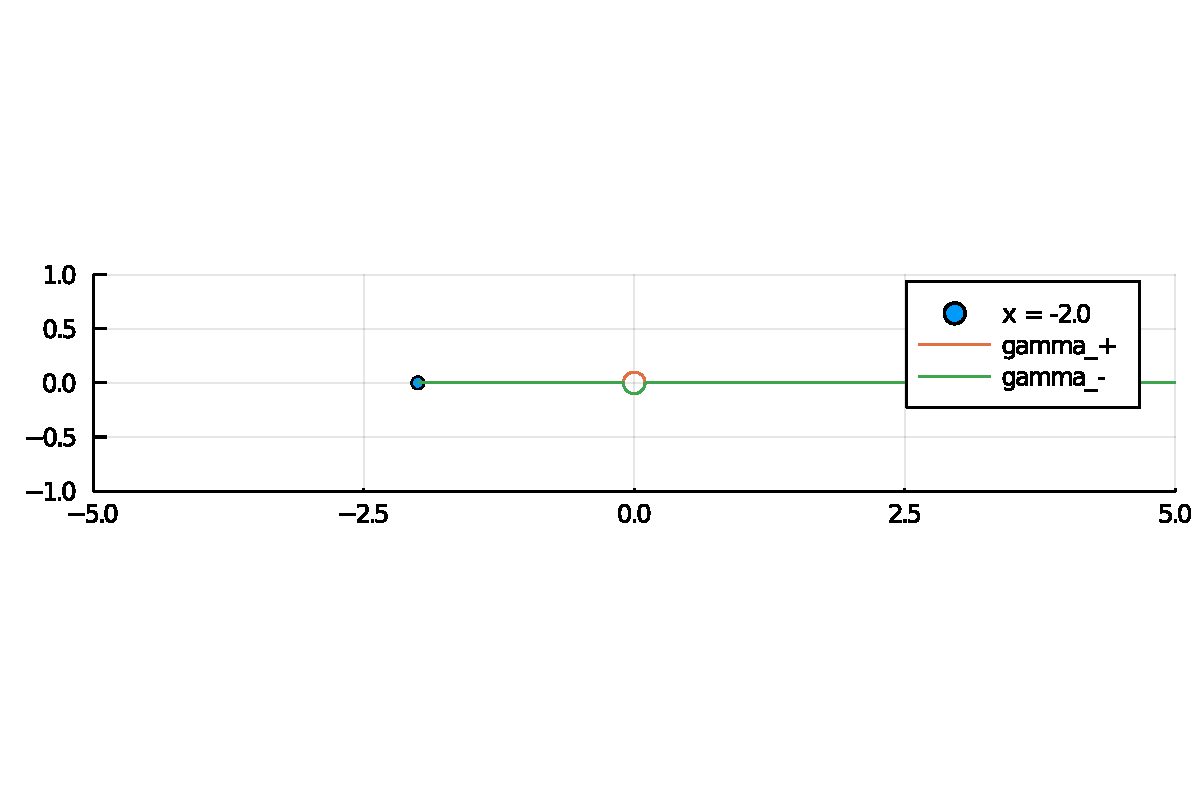
\includegraphics[width=\linewidth]{C:/Users/mfaso/OneDrive/Documents/GitHub/M3M6AppliedComplexAnalysis/output/figures/Solutions5_6_1.pdf}

So that

\[
\Gamma_\pm(\alpha, x) = \int_{\gamma_{\pm x}} \zeta^{\alpha-1} \E^{-\zeta} \D \zeta
\]
Note that

\[
\int_x^{-r} (\zeta_+^{\alpha - 1} - \E^{2 \I \pi \alpha} \zeta_-^{\alpha -1}) \E^{-\zeta} \D\zeta = 0
\]
since $\zeta_+^{\alpha-1} = \E^{\pi \I (\alpha-1)}|\zeta|^{\alpha-1} = \E^{2 \I \pi \alpha} \zeta_-^{\alpha-1}$. Furthermore, the integrals over the arcs tend to zero as $r \rightarrow 0$:

\[
|\I r^\alpha \int_0^\pi \E^{- r \E^{\I \theta}} \E^{\I \theta \alpha} \D \theta  | \leq r^\alpha \pi \E^r  \rightarrow 0
\]
and similarly on the lower arc. Thus we have


\begin{align*}
\Gamma_+(\alpha, x)-\E^{2 \I \pi \alpha} \Gamma_-(\alpha, x) &= \lim_{r \rightarrow 0 } \left(\int_{\gamma_{+x}} - \E^{2 \I \pi \alpha} \int_{\gamma_{-x}}\right) \zeta^{\alpha-1} \E^{-\zeta} \D \zeta \ccr
 = (1 - \E^{2 \I \pi \alpha})\int_0^\infty x^{\alpha-1} \E^{-x} \dx = (1 - \E^{2 \I \pi \alpha})\Gamma(\alpha)
\end{align*}
Note that, for $0 < \alpha < 1$,

\[
    \psi(z) = z^{-\alpha} \E^z \Gamma(\alpha, z)
\]
has the following properties:

\begin{itemize}
\item[1. ] \[
\psi(z)
\]
decays as $z \rightarrow \infty$, via integration by parts:

\end{itemize}
\[
    z^{-\alpha} \E^z \int_z^\infty \zeta^{\alpha-1} \E^{-\zeta} \D \zeta =
    z^{-1}  + z^{-\alpha} \int_z^\infty \zeta^{\alpha-2} \E^{z-\zeta} \D \zeta
\]
and we have assuming $z$ is bounded away from the negative real axis:

\[
\left\vert\int_z^\infty \zeta^{\alpha-2} \E^{z-\zeta} \D \zeta\right\vert \leq \int_z^\infty |\zeta|^{\alpha-2} \D \zeta = \int_0^\infty |x+z|^{\alpha-2} \D x  < \infty
\]
(otherwise one would use a deformed contour).

\begin{itemize}
\item[2. ] We have the subtractive jump:

\end{itemize}

\begin{align*}
\psi_+(x) - \psi_-(x) &= \E^x(x_+^{-\alpha} \Gamma_+(\alpha, x) -  x_-^{-\alpha}\Gamma_-(\alpha, x)) \ccr
= \E^x |x|^\alpha (\E^{-\I \pi \alpha} \Gamma_+(\alpha, z) - \E^{\I \pi \alpha} \Gamma_-(\alpha,x)) \ccr
 = \E^x |x|^\alpha \E^{-\I \pi \alpha} (1-\E^{2 \I \pi \alpha})
\end{align*}
We use these properties to verify that

\[
\CC[\diamond^\alpha \E^{-\diamond}](z) = {1 \over \Gamma(-\alpha)} {(-z)^\alpha \E^{-z} \Gamma(-\alpha, - z) \over
  \E^{-\I\pi\alpha} - \E^{\I\pi\alpha}}
\]
via Plemelj.


\begin{lstlisting}
(*@\HLJLn{x}@*) (*@\HLJLoB{=}@*) (*@\HLJLnf{Fun}@*)(*@\HLJLp{(}@*)(*@\HLJLni{0}@*) (*@\HLJLoB{..}@*) (*@\HLJLnfB{20.0}@*)(*@\HLJLp{)}@*)
(*@\HLJLn{\ensuremath{\alpha}}@*) (*@\HLJLoB{=}@*) (*@\HLJLoB{-}@*)(*@\HLJLnfB{0.1}@*)
(*@\HLJLn{z}@*) (*@\HLJLoB{=}@*) (*@\HLJLnfB{2.0}@*)(*@\HLJLoB{+}@*)(*@\HLJLn{im}@*)
(*@\HLJLnf{cauchy}@*)(*@\HLJLp{(}@*)(*@\HLJLn{x}@*)(*@\HLJLoB{{\textasciicircum}}@*)(*@\HLJLn{\ensuremath{\alpha}}@*)(*@\HLJLoB{*}@*)(*@\HLJLnf{exp}@*)(*@\HLJLp{(}@*)(*@\HLJLoB{-}@*)(*@\HLJLn{x}@*)(*@\HLJLp{),}@*) (*@\HLJLn{z}@*)(*@\HLJLp{)}@*)

(*@\HLJLn{\ensuremath{\Gamma}}@*) (*@\HLJLoB{=}@*) (*@\HLJLp{(}@*)(*@\HLJLn{\ensuremath{\alpha}}@*)(*@\HLJLp{,}@*)(*@\HLJLn{z}@*)(*@\HLJLp{)}@*) (*@\HLJLoB{->}@*) (*@\HLJLk{let}@*) (*@\HLJLn{\ensuremath{\zeta}}@*) (*@\HLJLoB{=}@*) (*@\HLJLn{z}@*) (*@\HLJLoB{+}@*) (*@\HLJLnf{Fun}@*)(*@\HLJLp{(}@*)(*@\HLJLni{0}@*) (*@\HLJLoB{..}@*) (*@\HLJLnfB{500.0}@*)(*@\HLJLp{)}@*)
    (*@\HLJLnf{linesum}@*)(*@\HLJLp{(}@*)(*@\HLJLn{\ensuremath{\zeta}}@*)(*@\HLJLoB{{\textasciicircum}}@*)(*@\HLJLp{(}@*)(*@\HLJLn{\ensuremath{\alpha}}@*)(*@\HLJLoB{-}@*)(*@\HLJLni{1}@*)(*@\HLJLp{)}@*)(*@\HLJLoB{*}@*)(*@\HLJLnf{exp}@*)(*@\HLJLp{(}@*)(*@\HLJLoB{-}@*)(*@\HLJLn{\ensuremath{\zeta}}@*)(*@\HLJLp{))}@*)
(*@\HLJLk{end}@*)

(*@\HLJLoB{-}@*)(*@\HLJLp{(}@*)(*@\HLJLoB{-}@*)(*@\HLJLn{z}@*)(*@\HLJLp{)}@*)(*@\HLJLoB{{\textasciicircum}}@*)(*@\HLJLn{\ensuremath{\alpha}}@*)(*@\HLJLoB{*}@*)(*@\HLJLnf{exp}@*)(*@\HLJLp{(}@*)(*@\HLJLoB{-}@*)(*@\HLJLn{z}@*)(*@\HLJLp{)}@*)(*@\HLJLnf{\ensuremath{\Gamma}}@*)(*@\HLJLp{(}@*)(*@\HLJLoB{-}@*)(*@\HLJLn{\ensuremath{\alpha}}@*)(*@\HLJLp{,}@*)(*@\HLJLoB{-}@*)(*@\HLJLn{z}@*)(*@\HLJLp{)}@*)(*@\HLJLoB{/}@*)(*@\HLJLp{(}@*)(*@\HLJLnf{gamma}@*)(*@\HLJLp{(}@*)(*@\HLJLoB{-}@*)(*@\HLJLn{\ensuremath{\alpha}}@*)(*@\HLJLp{)}@*)(*@\HLJLoB{*}@*)(*@\HLJLp{(}@*)(*@\HLJLnf{exp}@*)(*@\HLJLp{(}@*)(*@\HLJLn{im}@*)(*@\HLJLoB{*}@*)(*@\HLJLn{\ensuremath{\pi}}@*)(*@\HLJLoB{*}@*)(*@\HLJLn{\ensuremath{\alpha}}@*)(*@\HLJLp{)}@*)(*@\HLJLoB{-}@*)(*@\HLJLnf{exp}@*)(*@\HLJLp{(}@*)(*@\HLJLoB{-}@*)(*@\HLJLn{im}@*)(*@\HLJLoB{*}@*)(*@\HLJLn{\ensuremath{\pi}}@*)(*@\HLJLoB{*}@*)(*@\HLJLn{\ensuremath{\alpha}}@*)(*@\HLJLp{)))}@*)
\end{lstlisting}

\begin{lstlisting}
0.07199876331505128 + 0.05850612396048847im
\end{lstlisting}


\subsection{Problem 3}
\subsubsection{Problem 3.1}
We know that $L[a(z)]^{-1} = L[a(z)^{-1}]$ hence it's really about the Laurent series of $a(z)^{-1}$. We see that the roots of $a(z)$ satisfy

\[
0 =z^2 a(z) = z^4 - 4z^2 + 1.
\]
Using the quadratic formula with $w = z^2$ we have

\[
w = 2 \pm \sqrt 3 \Rightarrow z = \pm \sqrt{2 \pm \sqrt 3}.
\]
Since $2 - \sqrt 3 < 1$ and $2 + \sqrt 3 > 1$ we have the factorisation

\[
a(z) = \underbrace{z^2 - z_+}_{\phi_+(z)} \underbrace{1 - z_-/z^2}_{\phi_-(z)}
\]
for $z_{\pm} = 2 \pm \sqrt3$. We can take the reciprocal of $\phi_{\pm}$ using Geometric series, that is


\begin{align*}
\phi_+(z)^{-1} &= -{1 \over z_+} {1 \over 1 - z^2/z_+}  \ccr
= -{1 \over z_+} - {z^2 \over z_+^2} - {z^4 \over z_+^3} - \cdots \ccr
\phi_-(z)^{-1} = {1 \over 1- z_- /z^2} = 1 + {z_- \over z^2} + {z_-^2 \over z^4} + \cdots
\end{align*}
Thus we have

\[
a(z)^{-1} = \phi_+(z)^{-1} \phi_-(z)^{-1} =  \sum_{k=-\infty}^\infty b_{2k} z^{2k}
\]
where for $k \geq 0$

\[
b_{2k} =- \sum_{j=0}^\infty {z_-^j \over z_+^{j+k+1}} = - {z_+^{-k-1} \over 1 - z_-/z_+}
\]
and for $k < 0$

\[
b_{2k} =- \sum_{j=0}^\infty {z_-^{j-k} \over z_+^{j+1}} = - {z_-^{-k} \over z_+ - z_-}
\]
These give the diagonals of $L[a(z)^{-1}]$.

\emph{Verification}

A \emph{circulant matrix} is an effective approximation to a Laurent matrix (for reasons beyond the scope of this course, though it intuitively follows since the DFT diagonalises all circulant matrices):


\begin{lstlisting}
(*@\HLJLk{using}@*) (*@\HLJLn{ToeplitzMatrices}@*)(*@\HLJLp{,}@*) (*@\HLJLn{ApproxFun}@*)(*@\HLJLp{,}@*) (*@\HLJLn{Plots}@*)(*@\HLJLp{,}@*) (*@\HLJLn{LinearAlgebra}@*)(*@\HLJLp{,}@*) (*@\HLJLn{ComplexPhasePortrait}@*)(*@\HLJLp{,}@*) (*@\HLJLn{SingularIntegralEquations}@*)

(*@\HLJLn{n}@*) (*@\HLJLoB{=}@*) (*@\HLJLni{6}@*)
(*@\HLJLn{L}@*) (*@\HLJLoB{=}@*) (*@\HLJLnf{Circulant}@*)(*@\HLJLp{([}@*)(*@\HLJLoB{-}@*)(*@\HLJLni{4}@*)(*@\HLJLp{;}@*) (*@\HLJLni{1}@*)(*@\HLJLp{;}@*) (*@\HLJLnf{zeros}@*)(*@\HLJLp{(}@*)(*@\HLJLn{n}@*)(*@\HLJLoB{-}@*)(*@\HLJLni{3}@*)(*@\HLJLp{);}@*) (*@\HLJLni{1}@*)(*@\HLJLp{])}@*)
\end{lstlisting}

\begin{lstlisting}
6(*@\ensuremath{\times}@*(6 ToeplitzMatrices.Circulant(*@{{\{}}@*)Float64,Complex(*@{{\{}}@*)Float64(*@{{\}}}@*)(*@{{\}}}@*):
 -4.0   1.0   0.0   0.0   0.0   1.0
  1.0  -4.0   1.0   0.0   0.0   0.0
  0.0   1.0  -4.0   1.0   0.0   0.0
  0.0   0.0   1.0  -4.0   1.0   0.0
  0.0   0.0   0.0   1.0  -4.0   1.0
  1.0   0.0   0.0   0.0   1.0  -4.0
\end{lstlisting}


Taking \texttt{n} large, the entries inverse of \texttt{L} approximates the true inverse $L[a(z)]^{-1}$:


\begin{lstlisting}
(*@\HLJLn{n}@*) (*@\HLJLoB{=}@*) (*@\HLJLni{1000}@*)
(*@\HLJLn{L}@*) (*@\HLJLoB{=}@*) (*@\HLJLnf{Circulant}@*)(*@\HLJLp{([}@*)(*@\HLJLoB{-}@*)(*@\HLJLni{4}@*)(*@\HLJLp{;}@*) (*@\HLJLni{1}@*)(*@\HLJLp{;}@*) (*@\HLJLnf{zeros}@*)(*@\HLJLp{(}@*)(*@\HLJLn{n}@*)(*@\HLJLoB{-}@*)(*@\HLJLni{3}@*)(*@\HLJLp{);}@*) (*@\HLJLni{1}@*)(*@\HLJLp{])}@*)
(*@\HLJLnf{inv}@*)(*@\HLJLp{(}@*)(*@\HLJLn{L}@*)(*@\HLJLp{)}@*)
\end{lstlisting}

\begin{lstlisting}
1000(*@\ensuremath{\times}@*(1000 ToeplitzMatrices.Circulant(*@{{\{}}@*)Float64,Complex(*@{{\{}}@*)Float64(*@{{\}}}@*)(*@{{\}}}@*):
 -0.288675     -0.0773503    -0.0207259    (*@\ensuremath{\ldots}@*(  -0.0207259    -0.0773503
 -0.0773503    -0.288675     -0.0773503       -0.0055535    -0.0207259
 -0.0207259    -0.0773503    -0.288675        -0.00148806   -0.0055535
 -0.0055535    -0.0207259    -0.0773503       -0.000398723  -0.00148806
 -0.00148806   -0.0055535    -0.0207259       -0.000106838  -0.000398723
 -0.000398723  -0.00148806   -0.0055535    (*@\ensuremath{\ldots}@*(  -2.8627e-5    -0.000106838
 -0.000106838  -0.000398723  -0.00148806      -7.67059e-6   -2.8627e-5
 -2.8627e-5    -0.000106838  -0.000398723     -2.05533e-6   -7.67059e-6
 -7.67059e-6   -2.8627e-5    -0.000106838     -5.50724e-7   -2.05533e-6
 -2.05533e-6   -7.67059e-6   -2.8627e-5       -1.47566e-7   -5.50724e-7
  (*@\ensuremath{\vdots}@*(                                        (*@\ensuremath{\ddots}@*(                
 -2.05533e-6   -5.50724e-7   -1.47566e-7      -2.8627e-5    -7.67059e-6
 -7.67059e-6   -2.05533e-6   -5.50724e-7      -0.000106838  -2.8627e-5
 -2.8627e-5    -7.67059e-6   -2.05533e-6      -0.000398723  -0.000106838
 -0.000106838  -2.8627e-5    -7.67059e-6      -0.00148806   -0.000398723
 -0.000398723  -0.000106838  -2.8627e-5    (*@\ensuremath{\ldots}@*(  -0.0055535    -0.00148806
 -0.00148806   -0.000398723  -0.000106838     -0.0207259    -0.0055535
 -0.0055535    -0.00148806   -0.000398723     -0.0773503    -0.0207259
 -0.0207259    -0.0055535    -0.00148806      -0.288675     -0.0773503
 -0.0773503    -0.0207259    -0.0055535       -0.0773503    -0.288675
\end{lstlisting}


We verify this approximates the true inverse we deduced above by comparing the first few entries:


\begin{lstlisting}
(*@\HLJLn{zp}@*) (*@\HLJLoB{=}@*) (*@\HLJLni{2}@*)(*@\HLJLoB{+}@*)(*@\HLJLnf{sqrt}@*)(*@\HLJLp{(}@*)(*@\HLJLni{3}@*)(*@\HLJLp{)}@*)
(*@\HLJLn{zm}@*) (*@\HLJLoB{=}@*) (*@\HLJLni{2}@*)(*@\HLJLoB{-}@*)(*@\HLJLnf{sqrt}@*)(*@\HLJLp{(}@*)(*@\HLJLni{3}@*)(*@\HLJLp{)}@*)
(*@\HLJLoB{-}@*)(*@\HLJLn{zp}@*)(*@\HLJLoB{.{\textasciicircum}}@*)(*@\HLJLp{(}@*)(*@\HLJLoB{-}@*)(*@\HLJLp{(}@*)(*@\HLJLni{0}@*)(*@\HLJLoB{:}@*)(*@\HLJLni{4}@*)(*@\HLJLp{)}@*)(*@\HLJLoB{.-}@*)(*@\HLJLni{1}@*)(*@\HLJLp{)}@*) (*@\HLJLoB{/}@*) (*@\HLJLp{(}@*)(*@\HLJLni{1}@*)(*@\HLJLoB{-}@*)(*@\HLJLn{zm}@*)(*@\HLJLoB{/}@*)(*@\HLJLn{zp}@*)(*@\HLJLp{),}@*) (*@\HLJLnf{inv}@*)(*@\HLJLp{(}@*)(*@\HLJLn{L}@*)(*@\HLJLp{)[}@*)(*@\HLJLni{1}@*)(*@\HLJLp{,}@*)(*@\HLJLni{1}@*)(*@\HLJLoB{:}@*)(*@\HLJLni{5}@*)(*@\HLJLp{]}@*)
\end{lstlisting}

\begin{lstlisting}
([-0.28867513459481287, -0.07735026918962577, -0.02072594216369018, -0.0055
5349946513494, -0.001488055696849579], [-0.2886751345948129, -0.07735026918
962576, -0.020725942163690177, -0.005553499465134939, -0.001488055696849576
])
\end{lstlisting}


\subsection{Problem 3.2}
This part was solved as part of Problem 3.1.

\subsection{Problem 3.3}
Note that

\[
T[a(z)] = \sopmatrix{
-4 & 0 & 1 \\
0 & -4 & 0 & 1 \\
1 & 0 & -4 & 0 & 1 \\
& 1& 0 & -4 & 0 & 1 \\
&&\ddots &\ddots &\ddots &\ddots &\ddots
}
\]
The UL decomposition is $T[\phi_-] T[\phi_+]$, i.e., for $z_{\pm} = 2 \pm \sqrt3$,

\[
\underbrace{\sopmatrix{
1 & 0 & -z_- \\
& 1 & 0 & -z_- \\
&&\ddots & \ddots & \ddots
}}_U
\underbrace{\sopmatrix{-z_+ \\
0 & -z_+ \\
1 & 0 & -z_+ \\
& 1 & 0 & -z_+ \\
&&\ddots & \ddots & \ddots
}}_L
\]
\emph{Verification}


\begin{lstlisting}
(*@\HLJLn{n}@*) (*@\HLJLoB{=}@*) (*@\HLJLni{10}@*)
(*@\HLJLn{U}@*) (*@\HLJLoB{=}@*) (*@\HLJLnf{Toeplitz}@*)(*@\HLJLp{([}@*)(*@\HLJLni{1}@*)(*@\HLJLp{;}@*) (*@\HLJLnf{zeros}@*)(*@\HLJLp{(}@*)(*@\HLJLn{n}@*)(*@\HLJLoB{-}@*)(*@\HLJLni{1}@*)(*@\HLJLp{)],}@*) (*@\HLJLp{[}@*)(*@\HLJLni{1}@*)(*@\HLJLp{;}@*) (*@\HLJLni{0}@*)(*@\HLJLp{;}@*) (*@\HLJLoB{-}@*)(*@\HLJLn{zm}@*)(*@\HLJLp{;}@*) (*@\HLJLnf{zeros}@*)(*@\HLJLp{(}@*)(*@\HLJLn{n}@*)(*@\HLJLoB{-}@*)(*@\HLJLni{3}@*)(*@\HLJLp{)])}@*)
(*@\HLJLn{L}@*) (*@\HLJLoB{=}@*) (*@\HLJLnf{Toeplitz}@*)(*@\HLJLp{([}@*)(*@\HLJLoB{-}@*)(*@\HLJLn{zp}@*)(*@\HLJLp{;}@*) (*@\HLJLni{0}@*)(*@\HLJLp{;}@*) (*@\HLJLni{1}@*)(*@\HLJLp{;}@*) (*@\HLJLnf{zeros}@*)(*@\HLJLp{(}@*)(*@\HLJLn{n}@*)(*@\HLJLoB{-}@*)(*@\HLJLni{3}@*)(*@\HLJLp{)],}@*) (*@\HLJLp{[}@*)(*@\HLJLoB{-}@*)(*@\HLJLn{zp}@*)(*@\HLJLp{;}@*) (*@\HLJLnf{zeros}@*)(*@\HLJLp{(}@*)(*@\HLJLn{n}@*)(*@\HLJLoB{-}@*)(*@\HLJLni{1}@*)(*@\HLJLp{)])}@*)
(*@\HLJLn{U}@*)(*@\HLJLoB{*}@*)(*@\HLJLn{L}@*)
\end{lstlisting}

\begin{lstlisting}
10(*@\ensuremath{\times}@*(10 Array(*@{{\{}}@*)Float64,2(*@{{\}}}@*):
 -4.0   0.0   1.0   0.0   0.0   0.0   0.0   0.0   0.0       0.0
  0.0  -4.0   0.0   1.0   0.0   0.0   0.0   0.0   0.0       0.0
  1.0   0.0  -4.0   0.0   1.0   0.0   0.0   0.0   0.0       0.0
  0.0   1.0   0.0  -4.0   0.0   1.0   0.0   0.0   0.0       0.0
  0.0   0.0   1.0   0.0  -4.0   0.0   1.0   0.0   0.0       0.0
  0.0   0.0   0.0   1.0   0.0  -4.0   0.0   1.0   0.0       0.0
  0.0   0.0   0.0   0.0   1.0   0.0  -4.0   0.0   1.0       0.0
  0.0   0.0   0.0   0.0   0.0   1.0   0.0  -4.0   0.0       1.0
  0.0   0.0   0.0   0.0   0.0   0.0   1.0   0.0  -3.73205   0.0
  0.0   0.0   0.0   0.0   0.0   0.0   0.0   1.0   0.0      -3.73205
\end{lstlisting}


\subsection{Problem 3.4}
We have (see Problem 3.1)

\[
T[a(z)]^{-1} = L^{-1} U^{-1} =
\sopmatrix{-z_+^{-1} \\
0 & -z_+^{-1} \\
-z_+^{-2} & 0 & -z_+^{-1} \\
0 & -z_+^{-2} & 0 & -z_+^{-1} \\
-z_+^{-3} & 0 & -z_+^{-2} & 0 & -z_+^{-1} \\
&&\ddots & \ddots & \ddots
}
\sopmatrix{
1 & 0 & z_- & 0 &z_-^2 & 0 & \cdots \\
& 1 & 0 & z_- & 0 &z_-^2 & \cdots \\
& & 1 & 0 & z_- & 0 & \cdots \\
&&&\ddots & \ddots & \ddots
}
\]
\emph{Verification} For large \texttt{n} the entries of the inverse of Toeplitz matrix approximate those of the infinite-dimensional Toeplitz operator:


\begin{lstlisting}
(*@\HLJLn{n}@*) (*@\HLJLoB{=}@*) (*@\HLJLni{1000}@*)
(*@\HLJLn{T}@*) (*@\HLJLoB{=}@*) (*@\HLJLnf{Toeplitz}@*)(*@\HLJLp{([}@*)(*@\HLJLoB{-}@*)(*@\HLJLni{4}@*)(*@\HLJLp{;}@*) (*@\HLJLni{0}@*)(*@\HLJLp{;}@*) (*@\HLJLni{1}@*)(*@\HLJLp{;}@*) (*@\HLJLnf{zeros}@*)(*@\HLJLp{(}@*)(*@\HLJLn{n}@*)(*@\HLJLoB{-}@*)(*@\HLJLni{3}@*)(*@\HLJLp{)],}@*) (*@\HLJLp{[}@*)(*@\HLJLoB{-}@*)(*@\HLJLni{4}@*)(*@\HLJLp{;}@*) (*@\HLJLni{0}@*)(*@\HLJLp{;}@*) (*@\HLJLni{1}@*)(*@\HLJLp{;}@*) (*@\HLJLnf{zeros}@*)(*@\HLJLp{(}@*)(*@\HLJLn{n}@*)(*@\HLJLoB{-}@*)(*@\HLJLni{3}@*)(*@\HLJLp{)])}@*)
(*@\HLJLnf{inv}@*)(*@\HLJLp{(}@*)(*@\HLJLnf{Matrix}@*)(*@\HLJLp{(}@*)(*@\HLJLn{T}@*)(*@\HLJLp{))}@*)
\end{lstlisting}

\begin{lstlisting}
1000(*@\ensuremath{\times}@*(1000 Array(*@{{\{}}@*)Float64,2(*@{{\}}}@*):
 -0.267949      -0.0           -0.0717968     (*@\ensuremath{\ldots}@*(  -9.85983e-287  -0.0
  0.0           -0.267949      -0.0              -0.0           -9.85983e-2
87
 -0.0717968      0.0           -0.287187         -3.94393e-286  -0.0
  0.0           -0.0717968      0.0              -0.0           -3.94393e-2
86
 -0.0192379      0.0           -0.0769515        -1.47897e-285  -0.0
  0.0           -0.0192379      0.0           (*@\ensuremath{\ldots}@*(  -0.0           -1.47897e-2
85
 -0.00515478     0.0           -0.0206191        -5.5215e-285   -0.0
  0.0           -0.00515478     0.0              -0.0           -5.5215e-28
5
 -0.00138122     0.0           -0.00552487       -2.0607e-284   -0.0
  0.0           -0.00138122     0.0              -0.0           -2.0607e-28
4
  (*@\ensuremath{\vdots}@*(                                           (*@\ensuremath{\ddots}@*(                 
  0.0           -2.0607e-284    0.0              -0.0           -0.00138122
 -5.5215e-285    0.0           -2.2086e-284      -0.00515478    -0.0
  0.0           -5.5215e-285    0.0              -0.0           -0.00515478
 -1.47897e-285   0.0           -5.9159e-285      -0.0192379     -0.0
  0.0           -1.47897e-285   0.0           (*@\ensuremath{\ldots}@*(  -0.0           -0.0192379
 -3.94393e-286   0.0           -1.57757e-285     -0.0717968     -0.0
  0.0           -3.94393e-286   0.0              -0.0           -0.0717968
 -9.85983e-287   0.0           -3.94393e-286     -0.267949      -0.0
  0.0           -9.85983e-287   0.0               0.0           -0.267949
\end{lstlisting}


This matches our construction:


\begin{lstlisting}
(*@\HLJLn{li}@*) (*@\HLJLoB{=}@*) (*@\HLJLnf{zeros}@*)(*@\HLJLp{(}@*)(*@\HLJLn{n}@*)(*@\HLJLp{)}@*) (*@\HLJLcs{{\#}}@*) (*@\HLJLcs{inv(L)}@*) (*@\HLJLcs{coefficients}@*)
(*@\HLJLn{li}@*)(*@\HLJLp{[}@*)(*@\HLJLni{1}@*)(*@\HLJLoB{:}@*)(*@\HLJLni{2}@*)(*@\HLJLoB{:}@*)(*@\HLJLk{end}@*)(*@\HLJLp{]}@*) (*@\HLJLoB{=}@*) (*@\HLJLoB{-}@*)(*@\HLJLn{zp}@*)(*@\HLJLoB{.{\textasciicircum}}@*)(*@\HLJLp{(}@*)(*@\HLJLoB{-}@*)(*@\HLJLp{(}@*)(*@\HLJLni{1}@*)(*@\HLJLoB{:}@*)(*@\HLJLp{(}@*)(*@\HLJLn{n}@*) (*@\HLJLoB{\ensuremath{\div}}@*) (*@\HLJLni{2}@*)(*@\HLJLp{)))}@*)
(*@\HLJLn{Li}@*) (*@\HLJLoB{=}@*) (*@\HLJLnf{Toeplitz}@*)(*@\HLJLp{(}@*)(*@\HLJLn{li}@*)(*@\HLJLp{,}@*) (*@\HLJLp{[}@*)(*@\HLJLn{li}@*)(*@\HLJLp{[}@*)(*@\HLJLni{1}@*)(*@\HLJLp{];}@*) (*@\HLJLnf{zeros}@*)(*@\HLJLp{(}@*)(*@\HLJLn{n}@*)(*@\HLJLoB{-}@*)(*@\HLJLni{1}@*)(*@\HLJLp{)])}@*)
\end{lstlisting}

\begin{lstlisting}
1000(*@\ensuremath{\times}@*(1000 ToeplitzMatrices.Toeplitz(*@{{\{}}@*)Float64,Complex(*@{{\{}}@*)Float64(*@{{\}}}@*)(*@{{\}}}@*):
 -0.267949       0.0           (*@\ensuremath{\ldots}@*(   0.0         0.0        0.0
  0.0           -0.267949          0.0         0.0        0.0
 -0.0717968      0.0               0.0         0.0        0.0
  0.0           -0.0717968         0.0         0.0        0.0
 -0.0192379      0.0               0.0         0.0        0.0
  0.0           -0.0192379     (*@\ensuremath{\ldots}@*(   0.0         0.0        0.0
 -0.00515478     0.0               0.0         0.0        0.0
  0.0           -0.00515478        0.0         0.0        0.0
 -0.00138122     0.0               0.0         0.0        0.0
  0.0           -0.00138122        0.0         0.0        0.0
  (*@\ensuremath{\vdots}@*(                            (*@\ensuremath{\ddots}@*(                         
  0.0           -2.06071e-284      0.0         0.0        0.0
 -5.52165e-285   0.0               0.0         0.0        0.0
  0.0           -5.52165e-285      0.0         0.0        0.0
 -1.47952e-285   0.0               0.0         0.0        0.0
  0.0           -1.47952e-285  (*@\ensuremath{\ldots}@*(   0.0         0.0        0.0
 -3.96437e-286   0.0               0.0         0.0        0.0
  0.0           -3.96437e-286     -0.267949    0.0        0.0
 -1.06225e-286   0.0               0.0        -0.267949   0.0
  0.0           -1.06225e-286     -0.0717968   0.0       -0.267949
\end{lstlisting}


\begin{lstlisting}
(*@\HLJLn{ui}@*) (*@\HLJLoB{=}@*) (*@\HLJLnf{zeros}@*)(*@\HLJLp{(}@*)(*@\HLJLn{n}@*)(*@\HLJLp{)}@*) (*@\HLJLcs{{\#}}@*) (*@\HLJLcs{inv(U)}@*) (*@\HLJLcs{coefficients}@*)
(*@\HLJLn{ui}@*)(*@\HLJLp{[}@*)(*@\HLJLni{1}@*)(*@\HLJLoB{:}@*)(*@\HLJLni{2}@*)(*@\HLJLoB{:}@*)(*@\HLJLk{end}@*)(*@\HLJLp{]}@*) (*@\HLJLoB{=}@*) (*@\HLJLn{zm}@*)(*@\HLJLoB{.{\textasciicircum}}@*)(*@\HLJLp{(}@*)(*@\HLJLni{0}@*)(*@\HLJLoB{:}@*)(*@\HLJLp{(}@*)(*@\HLJLn{n}@*) (*@\HLJLoB{\ensuremath{\div}}@*) (*@\HLJLni{2}@*)(*@\HLJLp{)}@*)(*@\HLJLoB{-}@*)(*@\HLJLni{1}@*)(*@\HLJLp{)}@*)
(*@\HLJLn{Ui}@*) (*@\HLJLoB{=}@*) (*@\HLJLnf{Toeplitz}@*)(*@\HLJLp{([}@*)(*@\HLJLn{ui}@*)(*@\HLJLp{[}@*)(*@\HLJLni{1}@*)(*@\HLJLp{];}@*) (*@\HLJLnf{zeros}@*)(*@\HLJLp{(}@*)(*@\HLJLn{n}@*)(*@\HLJLoB{-}@*)(*@\HLJLni{1}@*)(*@\HLJLp{)],}@*) (*@\HLJLn{ui}@*)(*@\HLJLp{)}@*)
\end{lstlisting}

\begin{lstlisting}
1000(*@\ensuremath{\times}@*(1000 ToeplitzMatrices.Toeplitz(*@{{\{}}@*)Float64,Complex(*@{{\{}}@*)Float64(*@{{\}}}@*)(*@{{\}}}@*):
 1.0  0.0  0.267949  0.0       0.0717968  (*@\ensuremath{\ldots}@*(  3.96437e-286  0.0
 0.0  1.0  0.0       0.267949  0.0           0.0           3.96437e-286
 0.0  0.0  1.0       0.0       0.267949      1.47952e-285  0.0
 0.0  0.0  0.0       1.0       0.0           0.0           1.47952e-285
 0.0  0.0  0.0       0.0       1.0           5.52165e-285  0.0
 0.0  0.0  0.0       0.0       0.0        (*@\ensuremath{\ldots}@*(  0.0           5.52165e-285
 0.0  0.0  0.0       0.0       0.0           2.06071e-284  0.0
 0.0  0.0  0.0       0.0       0.0           0.0           2.06071e-284
 0.0  0.0  0.0       0.0       0.0           7.69067e-284  0.0
 0.0  0.0  0.0       0.0       0.0           0.0           7.69067e-284
 (*@\ensuremath{\vdots}@*(                                        (*@\ensuremath{\ddots}@*(                
 0.0  0.0  0.0       0.0       0.0           0.0           0.00515478
 0.0  0.0  0.0       0.0       0.0           0.0192379     0.0
 0.0  0.0  0.0       0.0       0.0           0.0           0.0192379
 0.0  0.0  0.0       0.0       0.0           0.0717968     0.0
 0.0  0.0  0.0       0.0       0.0        (*@\ensuremath{\ldots}@*(  0.0           0.0717968
 0.0  0.0  0.0       0.0       0.0           0.267949      0.0
 0.0  0.0  0.0       0.0       0.0           0.0           0.267949
 0.0  0.0  0.0       0.0       0.0           1.0           0.0
 0.0  0.0  0.0       0.0       0.0           0.0           1.0
\end{lstlisting}


\begin{lstlisting}
(*@\HLJLn{Li}@*)(*@\HLJLoB{*}@*)(*@\HLJLn{Ui}@*)
\end{lstlisting}

\begin{lstlisting}
1000(*@\ensuremath{\times}@*(1000 Array(*@{{\{}}@*)Float64,2(*@{{\}}}@*):
 -0.267949       0.0           -0.0717968     (*@\ensuremath{\ldots}@*(  -1.06225e-286   0.0
  0.0           -0.267949       0.0               0.0           -1.06225e-2
86
 -0.0717968      0.0           -0.287187         -4.249e-286     0.0
  0.0           -0.0717968      0.0               0.0           -4.249e-286
 -0.0192379      0.0           -0.0769515        -1.59337e-285   0.0
  0.0           -0.0192379      0.0           (*@\ensuremath{\ldots}@*(   0.0           -1.59337e-2
85
 -0.00515478     0.0           -0.0206191        -5.94859e-285   0.0
  0.0           -0.00515478     0.0               0.0           -5.94859e-2
85
 -0.00138122     0.0           -0.00552487       -2.2201e-284    0.0
  0.0           -0.00138122     0.0               0.0           -2.2201e-28
4
  (*@\ensuremath{\vdots}@*(                                           (*@\ensuremath{\ddots}@*(                 
  0.0           -2.06071e-284   0.0               0.0           -0.00148806
 -5.52165e-285   0.0           -2.20866e-284     -0.0055535      0.0
  0.0           -5.52165e-285   0.0               0.0           -0.0055535
 -1.47952e-285   0.0           -5.91809e-285     -0.0207259      0.0
  0.0           -1.47952e-285   0.0           (*@\ensuremath{\ldots}@*(   0.0           -0.0207259
 -3.96437e-286   0.0           -1.58575e-285     -0.0773503      0.0
  0.0           -3.96437e-286   0.0               0.0           -0.0773503
 -1.06225e-286   0.0           -4.249e-286       -0.288675       0.0
  0.0           -1.06225e-286   0.0               0.0           -0.288675
\end{lstlisting}


Note the inverse of a Toeplitz operator/matrix is not Toeplitz, unlike the case of a Laurent operator / Circulant matrix.

\subsubsection{Problem 3.5}
This is somewhat a trick question as $a(z) = (z^2 + 3)/ (z^2 + 2)$ is analytic inside the unit circle, so $T[a(z)]$ is lower triangular and  therefore

\[
T[a(z)]^{-1} = T[a(z)^{-1}] = T[(z^2 + 2)/(z^2+3)]
\]
\subsection{Problem 4}
\subsubsection{Problem 4.1}
It is 1 since we go around the origin once. The easiest way to see this is by direct inspection, we want to solve:

\[
\underbrace{\sopmatrix{0 \\  1  \\ & 1 \\ && 1 \\ &&&\ddots}}_{T[z]} \Vectt[u_0,u_1,\dots] = \Vectt[f_0,f_1,\dots]
\]
But the first row is always zero. If $f_0= 0 $ we therefore have the solution $u_n = f_{n+1}$.

\subsubsection{Problem 4.2}
The winding number is $-1$.  We want to solve:

\[
\underbrace{\sopmatrix{0 &  1  \\ && 1 \\ &&& 1 \\ &&&&\ddots}}_{T[z^{-1}]} \Vectt[u_0,u_1,\dots] = \Vectt[f_0,f_1,\dots]
\]
Now we have the solution for any constant $c$ $u_0 = c, u_n = f_{n-1}$. In other words, $\vc e_0$ is in the kernel.

\subsection{Problem 4.3}
If $a(z)$ has winding number $\kappa$ then $z^{-k} a(z)$ has trivial winding number. Therefore we have

\[
z^{-k} a(z) = \phi_+(z) \phi_-(z)
\]
As usual we can now take logarithms to deduce:

\[
\log(a(z) z^{-k}) = \log \phi_+(z) + \log \phi_-(z)
\]
which by Plemelj implies


\begin{align*}
\phi_+(z) &= \E^{\CC_+[ \log ( \diamond^{-k} a)](z)} \ccr
\phi_+(z) = \E^{-\CC_-[ \log ( \diamond^{-k} a)](z)}
\end{align*}
\subsection{Problem 4.4}
Note that for $\kappa \geq 0$ that $P$ is lower triangular Toeplitz, therefore we have using the algebraic properties of triangular Toeplitz

\[
T[\phi_-] T[z^\kappa] T[\phi_+] = T[\phi_-] T[z^\kappa \phi_+] = T[\phi_- z^\kappa \phi_+] = T[a(z)]
\]
When $\kappa \leq 0$ then $P$ is upper triangular Toeplitz and so

\[
T[\phi_-] T[z^\kappa] T[\phi_+] = T[\phi_- z^\kappa] T[\phi_+] = T[\phi_- z^\kappa \phi_+] = T[a(z)].
\]
\subsection{Problem 4.5}
The first question is: what is the winding number? The straightforward way to compute is via residue calculus. That is, if we calculate


\begin{align*}
{1 \over 2 \pi \I} \oint_a {1 \over z} \D z &=
{1 \over 2 \pi \I} \oint_C {a'(z) \over a(z)} \D z =
{-1 \over  \pi \I} \oint_C {z \over  z^2 + 1/2} \D z \ccr
= -2 \pr(\Res_{z = -{\I \over \sqrt 2}} + \Res_{z = {\I \over\sqrt 2}}) {z \over z^2 + 1/2} =  -2.
\end{align*}
This is also intuitive since $z^2$ clearly goes around the origin twice counterclockwise, so does $2z^2 + 1$ as the shift by 1 is not enough to change anything, therefore $(2z^2 + 1)^{-1}$ goes around twice clockwise.

Note that

\[
z^2 a(z) = \underbrace{z^2 \over 2 z^2 + 1}_{\phi_-(z)}
\]
Is already analytic outside the unit circle so we have $L = I$ and thus the factorisation

\[
T[a(z)] = \underbrace{T[\phi_-]}_U \underbrace{T[z^{-2}]}_P
\]
From the Laurent expansion

\[
\phi_-(z)^{-1} = 2 + 1/z^2
\]
We can compute

\[
U^{-1} \vc e_0 = T[\phi_-^{-1}] \vc e_0 =  2\vc e_0
\]
The kernel of $P$ is $\vc e_0$ and $\vc e_1$. Thus putting everything together we get the rather boring answer

\[
\Vectt[c,d, 2, 0,0,0,\dots]
\]
where $c$ and $d$ are arbitrary constants.

\subsection{Problem 5}
\subsubsection{Problem 5.1}
To be analytic at all we need decay at either $\pm \infty$, this has neither so is not defined.

\subsubsection{Problem 5.2}
It has exponential decay in the right-half plane, therefore

\[
\E^{\gamma x} f(x) = {\E^{\gamma x } \over 1 + \E^x}
\]
has exponential decay at both $\pm \infty$, provided $0 < \gamma < 1$. Therefore, we can take the strip $0 < \Im s < 1$.  (Note in each case the contour for the inverse Fourier transform can be any contour in the domain of analyticity.)

We can verify this by exact computation using Residue calculus: for $0 < \Im s < 1$, we can integrate over a rectangle to get:

\[
\left(\int_{-R}^R + \int_R^{2\I \pi + R} +  \int_{2 \I \pi + R}^{2\I \pi - R} + \int_{2 \I \pi - R}^{-R} \right) {\E^{-\I s x} \over 1 + \E^x} \dx = 2 \pi \I \Res_{z = \I \pi } {\E^{-\I s z} \over 1 + \E^z} =
- 2 \pi \I \E^{\pi s}
\]
Note that

\[
{\E^{-\I s (R + \I t)} \over 1 + \E^{R + \I t}} =
{\E^{-\I R \Re s + R \Im s  + t} \over 1 + \E^{R + \I t}} \rightarrow 0
\]
and

\[
{\E^{-\I s (-R + \I t)} \over 1 + \E^{R + \I t}} =
{\E^{\I R \Re s - R \Im s + t} \over 1 + \E^{R + \I t}} \rightarrow 0
\]
uniformly in $t$ as $R \rightarrow \infty$, hence we deduce that

\[
\left(\int_{-\infty}^\infty  +  \int_{2 \I \pi + \infty}^{2\I \pi - \infty}\right) {\E^{-\I s x} \over 1 + \E^x} \dx  =
- 2 \pi \I \E^{\pi s}
\]
Now note that

\[
\int_{2 \I \pi + \infty}^{2\I \pi - \infty} {\E^{-\I s t} \over 1 + \E^t} \dt  = \int_{\infty}^{-\infty} {\E^{-\I s (x+2 \I \pi)} \over 1 + \E^x} \dx = -\E^{2 \pi s} \int_{-\infty}^\infty  {\E^{-\I s x} \over 1 + \E^x} \dx
\]
Therefore, we have

\[
\int_{-\infty}^\infty  {\E^{-\I s x} \over 1 + \E^x} \dx  = - 2 \I \pi {\E^{\pi s} \over 1 -\E^{2 \pi s}} = \I \pi {\rm csch}\, \pi x
\]
which has poles at $0$ and $\I$:


\begin{lstlisting}
(*@\HLJLnf{phaseplot}@*)(*@\HLJLp{(}@*)(*@\HLJLoB{-}@*)(*@\HLJLnfB{3..3}@*)(*@\HLJLp{,}@*) (*@\HLJLoB{-}@*)(*@\HLJLnfB{10..10}@*)(*@\HLJLp{,}@*) (*@\HLJLn{z}@*) (*@\HLJLoB{->}@*) (*@\HLJLni{1}@*)(*@\HLJLoB{/}@*)(*@\HLJLp{(}@*)(*@\HLJLni{1}@*)(*@\HLJLoB{+}@*)(*@\HLJLnf{exp}@*)(*@\HLJLp{(}@*)(*@\HLJLn{z}@*)(*@\HLJLp{)))}@*) (*@\HLJLcs{{\#}integrand}@*)
\end{lstlisting}

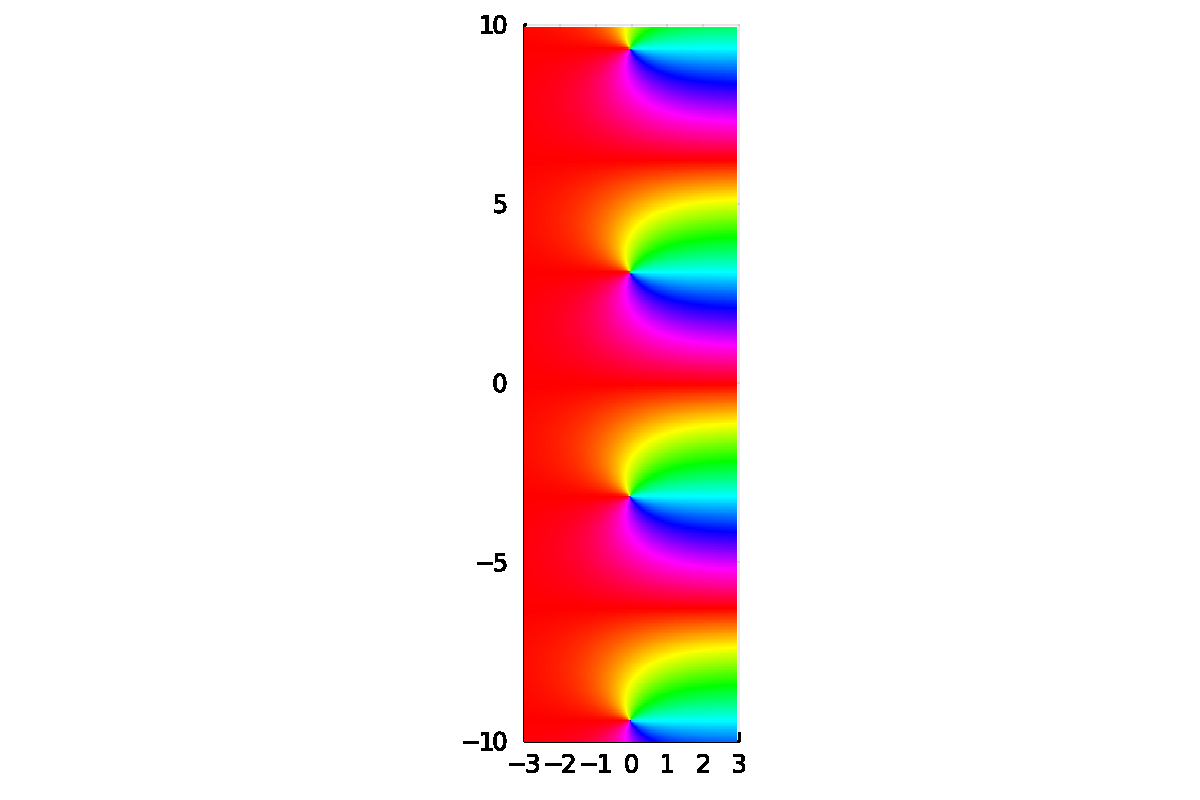
\includegraphics[width=\linewidth]{C:/Users/mfaso/OneDrive/Documents/GitHub/M3M6AppliedComplexAnalysis/output/figures/Solutions5_16_1.pdf}

\begin{lstlisting}
(*@\HLJLnf{phaseplot}@*)(*@\HLJLp{(}@*)(*@\HLJLoB{-}@*)(*@\HLJLnfB{3..3}@*)(*@\HLJLp{,}@*) (*@\HLJLoB{-}@*)(*@\HLJLnfB{3..3}@*)(*@\HLJLp{,}@*) (*@\HLJLn{z}@*) (*@\HLJLoB{->}@*) (*@\HLJLn{im}@*)(*@\HLJLoB{*}@*)(*@\HLJLn{\ensuremath{\pi}}@*)(*@\HLJLoB{*}@*)(*@\HLJLnf{csch}@*)(*@\HLJLp{(}@*)(*@\HLJLn{\ensuremath{\pi}}@*)(*@\HLJLoB{*}@*)(*@\HLJLn{z}@*)(*@\HLJLp{))}@*) (*@\HLJLcs{{\#}}@*) (*@\HLJLcs{transform}@*)
\end{lstlisting}

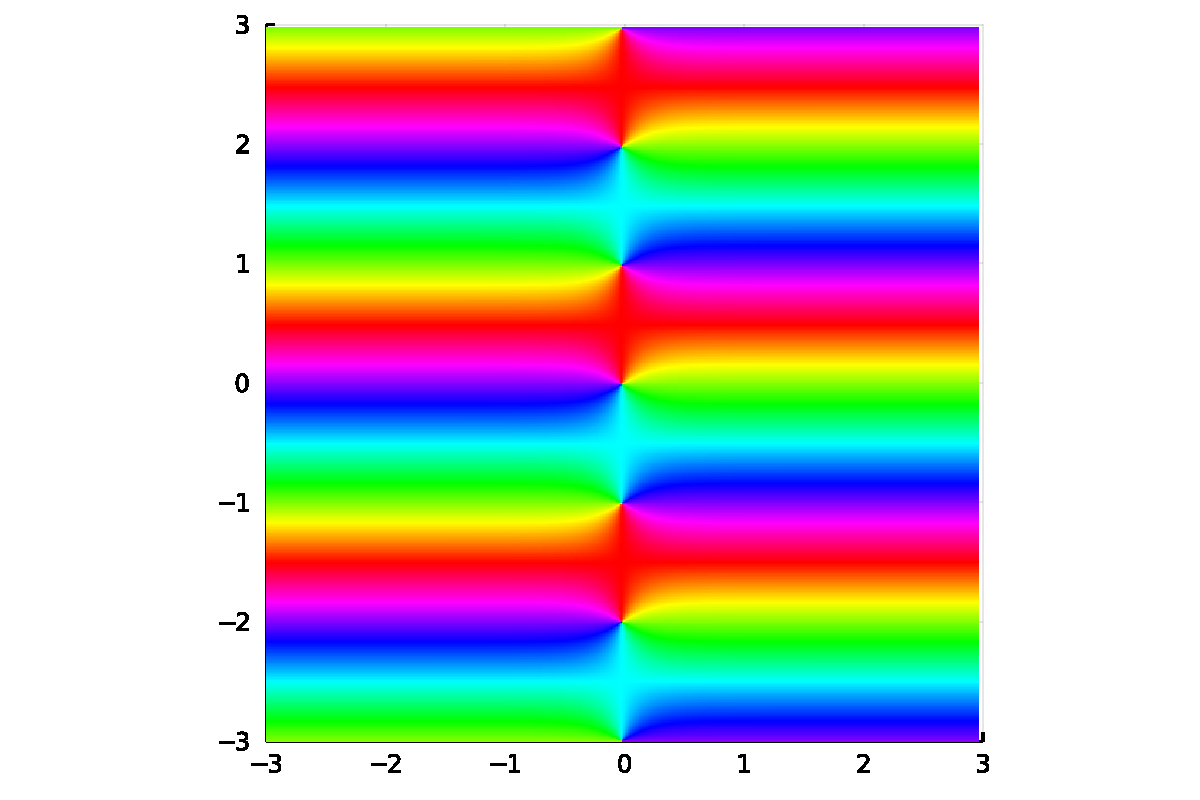
\includegraphics[width=\linewidth]{C:/Users/mfaso/OneDrive/Documents/GitHub/M3M6AppliedComplexAnalysis/output/figures/Solutions5_17_1.pdf}

\subsubsection{Problem 5.3}
Here $\E^{\gamma x } f(x) = \E^{(\gamma+2) x}$ has decay at $+\infty$ proved $\gamma < -2$, hence we have the strip $\Im s < -2$.

Indeed, its Fourier transform is

\[
-{\I \over 2 \I +s}
\]
by integration by parts.

\subsubsection{Problem 5.4}
Here it's $\Im s > 0$: unlike 1.1, we now have decay at $x \rightarrow \infty$ since $f_{\rm L}(x)$ is identically zero.

It's Fourier transform is determinable by integration-by-parts:

\[
\hat f(s) = \int_{-\infty}^0 x \E^{-\I s x} \dx = {1 \over \I s} \int_{-\infty}^0\E^{-\I s x} \dx = {1 \over s^2}
\]
\subsubsection{Problem 5.5}
The Fourier transforms are given above.

\subsubsection{Problem 5.6}
\[
\int_{-\infty}^\infty \delta(x) \E^{\I s x} \dx = 1
\]
It's actually an entire function, but non-decaying. This is hinting at the relationship between smoothness of a function and decay of its Fourier transform, and vice-versa: since $\delta(x)$ "decays" to all orders, we expect its Fourier transform to be entire, but since its not smooth at all, we expect no decay, so on a formal level we can predict the analyticity properties.

\subsection{Problem 6}
\subsubsection{Problem 6.1}
Note that

\[
K(z) =  {3\over 2} \E^{-|x|} \Rightarrow \hat K(s) = {3 \over 1+s^2}
\]
Provided $-1 < \Im s < 1$, and

\[
\widehat f_{\rm R}(s) = -{\I \over s} - {\alpha \over s^2}
\]
for $\Im s < 0$.  Define

\[
h(s) = - \widehat f_{\rm R}(s) = {\I \over s} + {\alpha \over s^2}
\]

\begin{lstlisting}
(*@\HLJLn{\ensuremath{\alpha}}@*) (*@\HLJLoB{=}@*) (*@\HLJLnfB{0.3}@*)
(*@\HLJLn{x}@*) (*@\HLJLoB{=}@*) (*@\HLJLnf{Fun}@*)(*@\HLJLp{(}@*)(*@\HLJLnfB{0..100}@*)(*@\HLJLp{)}@*)
(*@\HLJLn{f}@*) (*@\HLJLoB{=}@*) (*@\HLJLni{1}@*)  (*@\HLJLoB{+}@*) (*@\HLJLn{\ensuremath{\alpha}}@*)(*@\HLJLoB{*}@*)(*@\HLJLn{x}@*)
(*@\HLJLn{h}@*) (*@\HLJLoB{=}@*) (*@\HLJLn{s}@*) (*@\HLJLoB{->}@*) (*@\HLJLp{(}@*)(*@\HLJLn{im}@*)(*@\HLJLoB{/}@*)(*@\HLJLn{s}@*) (*@\HLJLoB{+}@*) (*@\HLJLn{\ensuremath{\alpha}}@*)(*@\HLJLoB{/}@*)(*@\HLJLn{s}@*)(*@\HLJLoB{{\textasciicircum}}@*)(*@\HLJLni{2}@*)(*@\HLJLp{)}@*)

(*@\HLJLn{\ensuremath{\gamma}}@*) (*@\HLJLoB{=}@*) (*@\HLJLoB{-}@*)(*@\HLJLnfB{0.5}@*) (*@\HLJLcs{{\#}}@*) (*@\HLJLcs{we}@*) (*@\HLJLcs{take}@*) (*@\HLJLcs{the}@*) (*@\HLJLcs{Fourier}@*) (*@\HLJLcs{transform}@*) (*@\HLJLcs{on}@*) (*@\HLJLcs{R}@*) (*@\HLJLcs{+}@*) (*@\HLJLcs{im*\ensuremath{\gamma}}@*)
(*@\HLJLn{s}@*) (*@\HLJLoB{=}@*) (*@\HLJLoB{-}@*)(*@\HLJLnfB{0.5}@*) (*@\HLJLoB{+}@*) (*@\HLJLn{im}@*)(*@\HLJLoB{*}@*)(*@\HLJLn{\ensuremath{\gamma}}@*)

(*@\HLJLoB{-}@*)(*@\HLJLnf{sum}@*)(*@\HLJLp{(}@*)(*@\HLJLn{f}@*)(*@\HLJLoB{*}@*)(*@\HLJLnf{exp}@*)(*@\HLJLp{(}@*)(*@\HLJLoB{-}@*)(*@\HLJLn{im}@*)(*@\HLJLoB{*}@*)(*@\HLJLn{s}@*)(*@\HLJLoB{*}@*)(*@\HLJLn{x}@*)(*@\HLJLp{))}@*) (*@\HLJLp{,}@*) (*@\HLJLnf{h}@*)(*@\HLJLp{(}@*)(*@\HLJLn{s}@*)(*@\HLJLp{)}@*)
\end{lstlisting}

\begin{lstlisting}
(-0.9999999999999862 - 1.5999999999999914im, -1.0 - 1.6im)
\end{lstlisting}


Transforming the equation, we have

\[
\Phi_+(s) - (1 + \hat K(s)) \Phi_-(s)  = {\I \over s} + {\alpha \over s^2}
\]
where

\[
1 + \hat K(s) = {4 + s^2 \over 1 + s^2} = {(s-2 \I) (s+2 \I) \over (s+\I)(s-\I)}
\]
This is very close to the example we did in lectures, so we already know the homogenous solution:

\[
\kappa(z) =  \begin{cases} {z + 2\I  \over z + \I}  & \Im z > \gamma \\
                            {z - \I  \over z - 2\I} & \Im z < \gamma
                            \end{cases}
\]
which is valid for $-1 < \gamma < 0$.


\begin{lstlisting}
(*@\HLJLn{g}@*) (*@\HLJLoB{=}@*) (*@\HLJLn{s}@*) (*@\HLJLoB{->}@*) (*@\HLJLp{(}@*)(*@\HLJLni{4}@*)(*@\HLJLoB{+}@*)(*@\HLJLn{s}@*)(*@\HLJLoB{{\textasciicircum}}@*)(*@\HLJLni{2}@*)(*@\HLJLp{)}@*)(*@\HLJLoB{/}@*)(*@\HLJLp{(}@*)(*@\HLJLni{1}@*)(*@\HLJLoB{+}@*)(*@\HLJLn{s}@*)(*@\HLJLoB{{\textasciicircum}}@*)(*@\HLJLni{2}@*)(*@\HLJLp{)}@*)

(*@\HLJLn{\ensuremath{\kappa}}@*) (*@\HLJLoB{=}@*) (*@\HLJLn{z}@*) (*@\HLJLoB{->}@*) (*@\HLJLnf{imag}@*)(*@\HLJLp{(}@*)(*@\HLJLn{z}@*)(*@\HLJLp{)}@*) (*@\HLJLoB{>}@*) (*@\HLJLn{\ensuremath{\gamma}}@*) (*@\HLJLoB{?}@*) (*@\HLJLp{(}@*)(*@\HLJLn{z}@*)(*@\HLJLoB{+}@*)(*@\HLJLn{im}@*)(*@\HLJLoB{*}@*)(*@\HLJLni{2}@*)(*@\HLJLp{)}@*)(*@\HLJLoB{/}@*)(*@\HLJLp{(}@*)(*@\HLJLn{z}@*)(*@\HLJLoB{+}@*)(*@\HLJLn{im}@*)(*@\HLJLp{)}@*) (*@\HLJLoB{:}@*)
                       (*@\HLJLp{(}@*)(*@\HLJLn{z}@*)(*@\HLJLoB{-}@*)(*@\HLJLn{im}@*)(*@\HLJLp{)}@*)(*@\HLJLoB{/}@*)(*@\HLJLp{(}@*)(*@\HLJLn{z}@*)(*@\HLJLoB{-}@*)(*@\HLJLn{im}@*)(*@\HLJLoB{*}@*)(*@\HLJLni{2}@*)(*@\HLJLp{)}@*)


(*@\HLJLnf{phaseplot}@*)(*@\HLJLp{(}@*)(*@\HLJLoB{-}@*)(*@\HLJLnfB{3..3}@*)(*@\HLJLp{,}@*) (*@\HLJLoB{-}@*)(*@\HLJLnfB{3..3}@*)(*@\HLJLp{,}@*) (*@\HLJLn{\ensuremath{\kappa}}@*)(*@\HLJLp{)}@*)
\end{lstlisting}

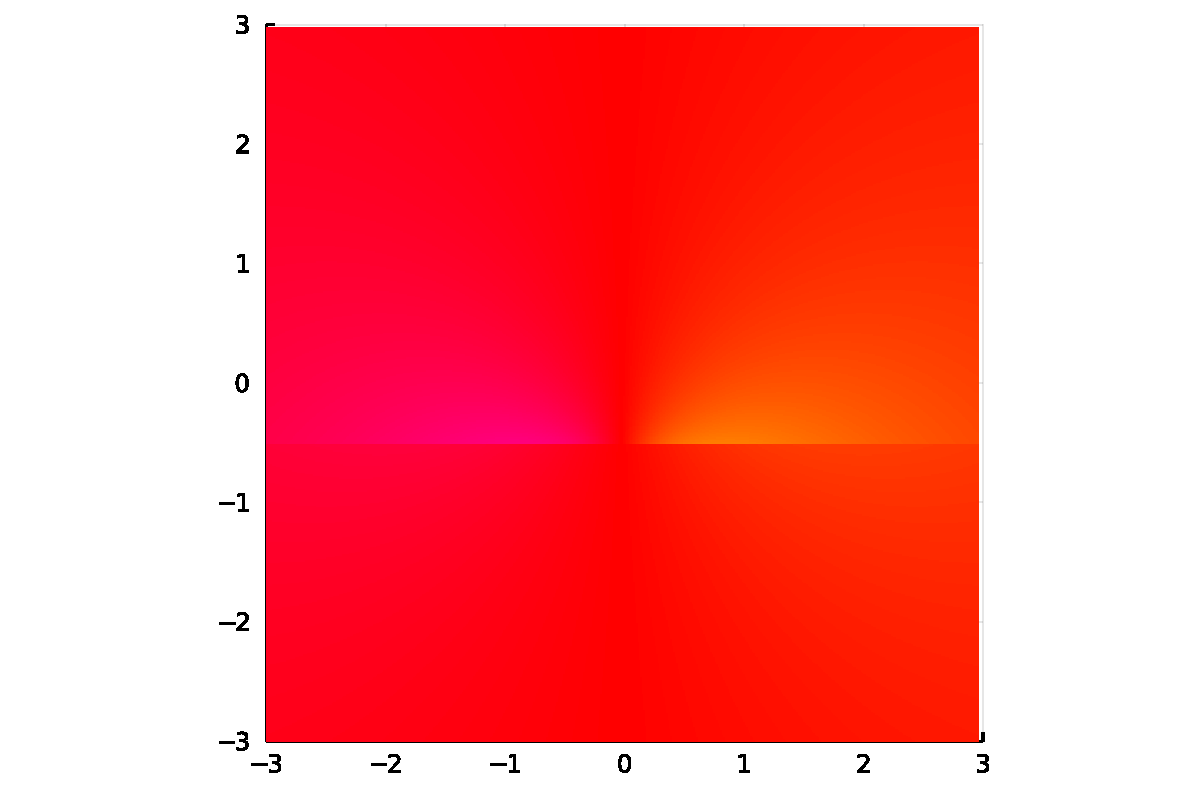
\includegraphics[width=\linewidth]{C:/Users/mfaso/OneDrive/Documents/GitHub/M3M6AppliedComplexAnalysis/output/figures/Solutions5_19_1.pdf}

\begin{lstlisting}
(*@\HLJLn{s}@*) (*@\HLJLoB{=}@*) (*@\HLJLnfB{0.1}@*) (*@\HLJLoB{+}@*) (*@\HLJLn{\ensuremath{\gamma}}@*)(*@\HLJLoB{*}@*)(*@\HLJLn{im}@*)
(*@\HLJLn{\ensuremath{\kappa}p}@*) (*@\HLJLoB{=}@*) (*@\HLJLnf{\ensuremath{\kappa}}@*)(*@\HLJLp{(}@*)(*@\HLJLn{s}@*) (*@\HLJLoB{+}@*) (*@\HLJLnf{eps}@*)(*@\HLJLp{()}@*)(*@\HLJLoB{*}@*)(*@\HLJLn{im}@*)(*@\HLJLp{)}@*)
(*@\HLJLn{\ensuremath{\kappa}m}@*) (*@\HLJLoB{=}@*) (*@\HLJLnf{\ensuremath{\kappa}}@*)(*@\HLJLp{(}@*)(*@\HLJLn{s}@*) (*@\HLJLoB{-}@*) (*@\HLJLnf{eps}@*)(*@\HLJLp{()}@*)(*@\HLJLoB{*}@*)(*@\HLJLn{im}@*)(*@\HLJLp{)}@*)

(*@\HLJLn{\ensuremath{\kappa}p}@*) (*@\HLJLoB{-}@*) (*@\HLJLn{\ensuremath{\kappa}m}@*)(*@\HLJLoB{*}@*)(*@\HLJLnf{g}@*)(*@\HLJLp{(}@*)(*@\HLJLn{s}@*)(*@\HLJLp{)}@*)
\end{lstlisting}

\begin{lstlisting}
-1.3322676295501878e-15 - 2.7755575615628914e-16im
\end{lstlisting}


We thus get the RH problem

\[
Y_+(s) - Y_-(s) = h(s)/\kappa_+(s) =  ({\I \over s} + {\alpha \over s^2})  {s + \I  \over s + 2 \I}
\]
We see this has poles at $0$ and $-2 \I$, so using partial fraction expansion we get

\[
({\I \over s} + {\alpha \over s^2})  {s + \I  \over s + \sqrt{3} \I} =
{\alpha \over 2 s^2}- {\I (\alpha-2) \over 4 s}  +{\I (2+\alpha) \over 4 (s+2 \I)}
\]
Therefore, splitting the poles between those above and below $\gamma$, we have

\[
Y(z) = \begin{cases}
 {\I (2+\alpha) \over 4 (z+2 \I)} & \Im z > \gamma \\
-{\alpha \over 2 z^2}+{\I (\alpha-2) \over 4 z} & \Im z < \gamma
\end{cases}
\]

\begin{lstlisting}
(*@\HLJLn{s}@*) (*@\HLJLoB{=}@*) (*@\HLJLnfB{0.1}@*) (*@\HLJLoB{+}@*) (*@\HLJLn{\ensuremath{\gamma}}@*)(*@\HLJLoB{*}@*)(*@\HLJLn{im}@*)
(*@\HLJLn{Y}@*) (*@\HLJLoB{=}@*) (*@\HLJLn{z}@*) (*@\HLJLoB{->}@*) (*@\HLJLnf{imag}@*)(*@\HLJLp{(}@*)(*@\HLJLn{z}@*)(*@\HLJLp{)}@*) (*@\HLJLoB{>}@*) (*@\HLJLn{\ensuremath{\gamma}}@*) (*@\HLJLoB{?}@*) (*@\HLJLn{im}@*)(*@\HLJLoB{*}@*)(*@\HLJLp{(}@*)(*@\HLJLni{2}@*)(*@\HLJLoB{+}@*)(*@\HLJLn{\ensuremath{\alpha}}@*)(*@\HLJLp{)}@*)(*@\HLJLoB{/}@*)(*@\HLJLp{(}@*)(*@\HLJLni{4}@*)(*@\HLJLoB{*}@*)(*@\HLJLp{(}@*)(*@\HLJLn{z}@*)(*@\HLJLoB{+}@*)(*@\HLJLni{2}@*)(*@\HLJLn{im}@*)(*@\HLJLp{))}@*) (*@\HLJLoB{:}@*)
                     (*@\HLJLoB{-}@*) (*@\HLJLn{\ensuremath{\alpha}}@*)(*@\HLJLoB{/}@*)(*@\HLJLp{(}@*)(*@\HLJLni{2}@*)(*@\HLJLn{z}@*)(*@\HLJLoB{{\textasciicircum}}@*)(*@\HLJLni{2}@*)(*@\HLJLp{)}@*) (*@\HLJLoB{+}@*) (*@\HLJLn{im}@*)(*@\HLJLoB{*}@*)(*@\HLJLp{(}@*)(*@\HLJLn{\ensuremath{\alpha}}@*)(*@\HLJLoB{-}@*)(*@\HLJLni{2}@*)(*@\HLJLp{)}@*)(*@\HLJLoB{/}@*)(*@\HLJLp{(}@*)(*@\HLJLni{4}@*)(*@\HLJLn{z}@*)(*@\HLJLp{)}@*)


(*@\HLJLn{Yp}@*) (*@\HLJLoB{=}@*) (*@\HLJLnf{Y}@*)(*@\HLJLp{(}@*)(*@\HLJLn{s}@*) (*@\HLJLoB{+}@*) (*@\HLJLnf{eps}@*)(*@\HLJLp{()}@*)(*@\HLJLoB{*}@*)(*@\HLJLn{im}@*)(*@\HLJLp{)}@*)
(*@\HLJLn{Ym}@*) (*@\HLJLoB{=}@*) (*@\HLJLnf{Y}@*)(*@\HLJLp{(}@*)(*@\HLJLn{s}@*) (*@\HLJLoB{-}@*) (*@\HLJLnf{eps}@*)(*@\HLJLp{()}@*)(*@\HLJLoB{*}@*)(*@\HLJLn{im}@*)(*@\HLJLp{)}@*)

(*@\HLJLn{Yp}@*) (*@\HLJLoB{-}@*) (*@\HLJLn{Ym}@*)  (*@\HLJLp{,}@*) (*@\HLJLnf{h}@*)(*@\HLJLp{(}@*)(*@\HLJLn{s}@*)(*@\HLJLp{)}@*)(*@\HLJLoB{/}@*)(*@\HLJLn{\ensuremath{\kappa}p}@*)
\end{lstlisting}

\begin{lstlisting}
(-0.9682149028643237 + 0.4107975074619046im, -0.9682149028643242 + 0.410797
507461905im)
\end{lstlisting}


We therefore have

\[
\Phi(z)  = \kappa(z) Y(z) = \begin{cases}
 {\I (2+\alpha) \over 4 (z+ \I)}  & \Im z > \gamma \\
(-{\alpha \over 2 z^2}+{\I (\alpha-2) \over 4 z}  ) {z - \I  \over z - 2\I} & \Im z < \gamma
\end{cases}
\]

\begin{lstlisting}
(*@\HLJLn{\ensuremath{\Phi}}@*) (*@\HLJLoB{=}@*) (*@\HLJLn{z}@*) (*@\HLJLoB{->}@*) (*@\HLJLnf{imag}@*)(*@\HLJLp{(}@*)(*@\HLJLn{z}@*)(*@\HLJLp{)}@*) (*@\HLJLoB{>}@*) (*@\HLJLn{\ensuremath{\gamma}}@*) (*@\HLJLoB{?}@*) (*@\HLJLn{im}@*)(*@\HLJLoB{*}@*)(*@\HLJLp{(}@*)(*@\HLJLni{2}@*)(*@\HLJLoB{+}@*)(*@\HLJLn{\ensuremath{\alpha}}@*)(*@\HLJLp{)}@*)(*@\HLJLoB{/}@*)(*@\HLJLp{(}@*)(*@\HLJLni{4}@*)(*@\HLJLoB{*}@*)(*@\HLJLp{(}@*)(*@\HLJLn{z}@*)(*@\HLJLoB{+}@*)(*@\HLJLn{im}@*)(*@\HLJLp{))}@*) (*@\HLJLoB{:}@*)
                      (*@\HLJLp{(}@*)(*@\HLJLoB{-}@*)(*@\HLJLn{\ensuremath{\alpha}}@*)(*@\HLJLoB{/}@*)(*@\HLJLp{(}@*)(*@\HLJLni{2}@*)(*@\HLJLn{z}@*)(*@\HLJLoB{{\textasciicircum}}@*)(*@\HLJLni{2}@*)(*@\HLJLp{)}@*) (*@\HLJLoB{+}@*) (*@\HLJLn{im}@*)(*@\HLJLoB{*}@*)(*@\HLJLp{(}@*)(*@\HLJLn{\ensuremath{\alpha}}@*)(*@\HLJLoB{-}@*)(*@\HLJLni{2}@*)(*@\HLJLp{)}@*)(*@\HLJLoB{/}@*)(*@\HLJLp{(}@*)(*@\HLJLni{4}@*)(*@\HLJLn{z}@*)(*@\HLJLp{))}@*)(*@\HLJLoB{*}@*)(*@\HLJLp{(}@*)(*@\HLJLn{z}@*)(*@\HLJLoB{-}@*)(*@\HLJLn{im}@*)(*@\HLJLp{)}@*)(*@\HLJLoB{/}@*)(*@\HLJLp{(}@*)(*@\HLJLn{z}@*)(*@\HLJLoB{-}@*)(*@\HLJLni{2}@*)(*@\HLJLn{im}@*)(*@\HLJLp{)}@*)
(*@\HLJLn{\ensuremath{\Phi}p}@*) (*@\HLJLoB{=}@*) (*@\HLJLnf{\ensuremath{\Phi}}@*)(*@\HLJLp{(}@*)(*@\HLJLn{s}@*)(*@\HLJLoB{+}@*)(*@\HLJLnf{eps}@*)(*@\HLJLp{()}@*)(*@\HLJLn{im}@*)(*@\HLJLp{)}@*)
(*@\HLJLn{\ensuremath{\Phi}m}@*) (*@\HLJLoB{=}@*) (*@\HLJLnf{\ensuremath{\Phi}}@*)(*@\HLJLp{(}@*)(*@\HLJLn{s}@*)(*@\HLJLoB{-}@*)(*@\HLJLnf{eps}@*)(*@\HLJLp{()}@*)(*@\HLJLn{im}@*)(*@\HLJLp{)}@*)

(*@\HLJLn{\ensuremath{\Phi}p}@*) (*@\HLJLoB{-}@*) (*@\HLJLn{\ensuremath{\Phi}m}@*)(*@\HLJLoB{*}@*)(*@\HLJLnf{g}@*)(*@\HLJLp{(}@*)(*@\HLJLn{s}@*)(*@\HLJLp{)}@*) (*@\HLJLp{,}@*) (*@\HLJLnf{h}@*)(*@\HLJLp{(}@*)(*@\HLJLn{s}@*)(*@\HLJLp{)}@*)
\end{lstlisting}

\begin{lstlisting}
(-2.9881656804733714 + 0.8284023668639042im, -2.9881656804733723 + 0.828402
3668639053im)
\end{lstlisting}


Finally, we recover the solution by inverting $\Phi_-$, using Residue calculus in the upper half plane: for $x > 0$ we have


\begin{align*}
u(x) &= {1 \over 2 \pi} \int_{-\infty+ \I \gamma}^{\infty + \I \gamma} (-{\alpha \over 2 z^2}+{\I (\alpha-2) \over 4 z}  ) {z - \I  \over z - 2\I}  \E^{\I z x}  \dz \\
&= \I (\Res_{z = 0} + \Res_{z = 2\I}) (-{\alpha \over 2 z^2}+{\I (\alpha-2) \over 4 z}  ) {z - \I  \over z - 2\I}  \E^{\I z x} = {1+x \alpha \over 4} - {\alpha+1 \over 4} \E^{-2 x}
\end{align*}
Did it work? yes:


\begin{lstlisting}
(*@\HLJLn{t}@*) (*@\HLJLoB{=}@*) (*@\HLJLnf{Fun}@*)(*@\HLJLp{(}@*)(*@\HLJLni{0}@*) (*@\HLJLoB{..}@*) (*@\HLJLni{50}@*)(*@\HLJLp{)}@*)
(*@\HLJLn{u}@*) (*@\HLJLoB{=}@*) (*@\HLJLp{(}@*)(*@\HLJLni{1}@*)(*@\HLJLoB{+}@*)(*@\HLJLn{t}@*)(*@\HLJLoB{*}@*)(*@\HLJLn{\ensuremath{\alpha}}@*)(*@\HLJLp{)}@*)(*@\HLJLoB{/}@*)(*@\HLJLni{4}@*) (*@\HLJLoB{-}@*) (*@\HLJLp{(}@*)(*@\HLJLn{\ensuremath{\alpha}}@*)(*@\HLJLoB{-}@*)(*@\HLJLni{1}@*)(*@\HLJLp{)}@*)(*@\HLJLoB{/}@*)(*@\HLJLni{4}@*)(*@\HLJLoB{*}@*)(*@\HLJLnf{exp}@*)(*@\HLJLp{(}@*)(*@\HLJLoB{-}@*)(*@\HLJLni{2}@*)(*@\HLJLn{t}@*)(*@\HLJLp{)}@*)
(*@\HLJLn{x}@*) (*@\HLJLoB{=}@*) (*@\HLJLnfB{0.1}@*)
(*@\HLJLnf{u}@*)(*@\HLJLp{(}@*)(*@\HLJLn{x}@*)(*@\HLJLp{)}@*) (*@\HLJLoB{+}@*) (*@\HLJLni{3}@*)(*@\HLJLoB{/}@*)(*@\HLJLni{2}@*)(*@\HLJLoB{*}@*)(*@\HLJLnf{sum}@*)(*@\HLJLp{(}@*)(*@\HLJLnf{exp}@*)(*@\HLJLp{(}@*)(*@\HLJLoB{-}@*)(*@\HLJLnf{abs}@*)(*@\HLJLp{(}@*)(*@\HLJLn{t}@*)(*@\HLJLoB{-}@*)(*@\HLJLn{x}@*)(*@\HLJLp{))}@*)(*@\HLJLoB{*}@*)(*@\HLJLn{u}@*)(*@\HLJLp{)}@*) (*@\HLJLp{,}@*) (*@\HLJLnf{f}@*)(*@\HLJLp{(}@*)(*@\HLJLn{x}@*)(*@\HLJLp{)}@*)
\end{lstlisting}

\begin{lstlisting}
(1.0300000000000025, 1.03)
\end{lstlisting}


\subsubsection{Problem 6.2}
Setting up the problem as above, we arrive at a degenerate RH problem:

\[
\Phi_+(s) - g(s) \Phi_-(s) = h(s)
\]
where

\[
g(s) = \widehat K(s) = {2\alpha \over \alpha^2 +s^2}= {2 \alpha \over (s-\I \alpha)(s+\I \alpha)}
\]
and

\[
h(s) = {\I \over s} + {\alpha \over s^2} = \I {s -\I \alpha \over s^2}
\]
Suppose we allow $\kappa_-(s) \sim s$ to have growth, then we can write

\[
\kappa(z) = \begin{cases} {1 \over z+\I \alpha }& \Im z > \gamma \\
                        {z-\I \alpha \over 2 \alpha} & \Im z < \gamma
\end{cases}
\]
so that

\[
\kappa_+(s) = \kappa_-(s) g(s)
\]

\begin{lstlisting}
(*@\HLJLn{\ensuremath{\alpha}}@*) (*@\HLJLoB{=}@*) (*@\HLJLnfB{0.3}@*)

(*@\HLJLn{g}@*) (*@\HLJLoB{=}@*) (*@\HLJLn{s}@*) (*@\HLJLoB{->}@*) (*@\HLJLp{(}@*)(*@\HLJLni{2}@*)(*@\HLJLn{\ensuremath{\alpha}}@*)(*@\HLJLp{)}@*)(*@\HLJLoB{/}@*)(*@\HLJLp{(}@*)(*@\HLJLn{\ensuremath{\alpha}}@*)(*@\HLJLoB{{\textasciicircum}}@*)(*@\HLJLni{2}@*)(*@\HLJLoB{+}@*)(*@\HLJLn{s}@*)(*@\HLJLoB{{\textasciicircum}}@*)(*@\HLJLni{2}@*)(*@\HLJLp{)}@*)
(*@\HLJLn{h}@*) (*@\HLJLoB{=}@*) (*@\HLJLn{s}@*) (*@\HLJLoB{->}@*) (*@\HLJLp{(}@*)(*@\HLJLn{im}@*)(*@\HLJLoB{/}@*)(*@\HLJLn{s}@*) (*@\HLJLoB{+}@*) (*@\HLJLn{\ensuremath{\alpha}}@*)(*@\HLJLoB{/}@*)(*@\HLJLn{s}@*)(*@\HLJLoB{{\textasciicircum}}@*)(*@\HLJLni{2}@*)(*@\HLJLp{)}@*)

(*@\HLJLn{\ensuremath{\kappa}}@*) (*@\HLJLoB{=}@*) (*@\HLJLn{z}@*) (*@\HLJLoB{->}@*) (*@\HLJLnf{imag}@*)(*@\HLJLp{(}@*)(*@\HLJLn{z}@*)(*@\HLJLp{)}@*) (*@\HLJLoB{>}@*) (*@\HLJLn{\ensuremath{\gamma}}@*) (*@\HLJLoB{?}@*) (*@\HLJLni{1}@*)(*@\HLJLoB{/}@*)(*@\HLJLp{(}@*)(*@\HLJLn{z}@*) (*@\HLJLoB{+}@*) (*@\HLJLn{im}@*)(*@\HLJLoB{*}@*)(*@\HLJLn{\ensuremath{\alpha}}@*)(*@\HLJLp{)}@*) (*@\HLJLoB{:}@*)
                       (*@\HLJLp{(}@*)(*@\HLJLn{z}@*)(*@\HLJLoB{-}@*)(*@\HLJLn{im}@*)(*@\HLJLoB{*}@*)(*@\HLJLn{\ensuremath{\alpha}}@*)(*@\HLJLp{)}@*)(*@\HLJLoB{/}@*)(*@\HLJLp{(}@*)(*@\HLJLni{2}@*)(*@\HLJLn{\ensuremath{\alpha}}@*)(*@\HLJLp{)}@*)

(*@\HLJLnf{phaseplot}@*)(*@\HLJLp{(}@*)(*@\HLJLoB{-}@*)(*@\HLJLnfB{3..3}@*)(*@\HLJLp{,}@*) (*@\HLJLoB{-}@*)(*@\HLJLnfB{3..3}@*)(*@\HLJLp{,}@*) (*@\HLJLn{\ensuremath{\kappa}}@*)(*@\HLJLp{)}@*)
\end{lstlisting}

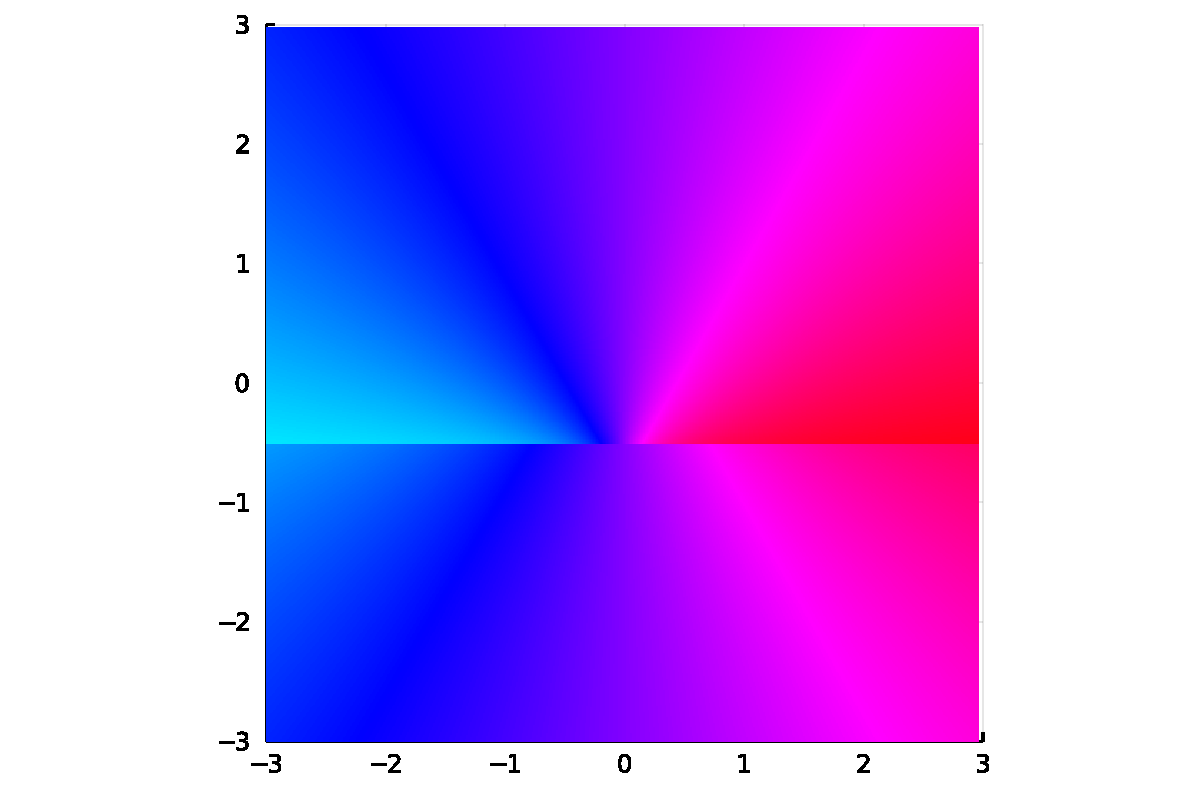
\includegraphics[width=\linewidth]{C:/Users/mfaso/OneDrive/Documents/GitHub/M3M6AppliedComplexAnalysis/output/figures/Solutions5_24_1.pdf}

\begin{lstlisting}
(*@\HLJLn{s}@*) (*@\HLJLoB{=}@*) (*@\HLJLnfB{0.1}@*) (*@\HLJLoB{+}@*) (*@\HLJLn{\ensuremath{\gamma}}@*)(*@\HLJLoB{*}@*)(*@\HLJLn{im}@*)
(*@\HLJLn{\ensuremath{\kappa}p}@*) (*@\HLJLoB{=}@*) (*@\HLJLnf{\ensuremath{\kappa}}@*)(*@\HLJLp{(}@*)(*@\HLJLn{s}@*) (*@\HLJLoB{+}@*) (*@\HLJLnf{eps}@*)(*@\HLJLp{()}@*)(*@\HLJLoB{*}@*)(*@\HLJLn{im}@*)(*@\HLJLp{)}@*)
(*@\HLJLn{\ensuremath{\kappa}m}@*) (*@\HLJLoB{=}@*) (*@\HLJLnf{\ensuremath{\kappa}}@*)(*@\HLJLp{(}@*)(*@\HLJLn{s}@*) (*@\HLJLoB{-}@*) (*@\HLJLnf{eps}@*)(*@\HLJLp{()}@*)(*@\HLJLoB{*}@*)(*@\HLJLn{im}@*)(*@\HLJLp{)}@*)

(*@\HLJLn{\ensuremath{\kappa}p}@*) (*@\HLJLp{,}@*) (*@\HLJLn{\ensuremath{\kappa}m}@*)(*@\HLJLoB{*}@*)(*@\HLJLnf{g}@*)(*@\HLJLp{(}@*)(*@\HLJLn{s}@*)(*@\HLJLp{)}@*)
\end{lstlisting}

\begin{lstlisting}
(2.0000000000000036 + 4.000000000000003im, 2.000000000000001 + 4.0000000000
00001im)
\end{lstlisting}


Then we have

\[
h(s)/\kappa_+(s) =  \I {s^2 + \alpha^2 \over s^2} = \I + \I {\alpha^2 \over s^2}
\]
and then we can write

\[
Y(z) = \begin{cases}
\I & \Im z > \gamma \\
-{\I \alpha^2 \over z^2} & \Im z < \gamma
\end{cases}
\]

\begin{lstlisting}
(*@\HLJLn{s}@*) (*@\HLJLoB{=}@*) (*@\HLJLnfB{0.1}@*) (*@\HLJLoB{+}@*) (*@\HLJLn{\ensuremath{\gamma}}@*)(*@\HLJLoB{*}@*)(*@\HLJLn{im}@*)
(*@\HLJLn{Y}@*) (*@\HLJLoB{=}@*) (*@\HLJLn{z}@*) (*@\HLJLoB{->}@*) (*@\HLJLnf{imag}@*)(*@\HLJLp{(}@*)(*@\HLJLn{z}@*)(*@\HLJLp{)}@*) (*@\HLJLoB{>}@*) (*@\HLJLn{\ensuremath{\gamma}}@*) (*@\HLJLoB{?}@*) (*@\HLJLn{im}@*) (*@\HLJLoB{:}@*)
                     (*@\HLJLoB{-}@*)(*@\HLJLn{im}@*)(*@\HLJLoB{*}@*)(*@\HLJLn{\ensuremath{\alpha}}@*)(*@\HLJLoB{{\textasciicircum}}@*)(*@\HLJLni{2}@*)(*@\HLJLoB{/}@*)(*@\HLJLn{s}@*)(*@\HLJLoB{{\textasciicircum}}@*)(*@\HLJLni{2}@*)


(*@\HLJLn{Yp}@*) (*@\HLJLoB{=}@*) (*@\HLJLnf{Y}@*)(*@\HLJLp{(}@*)(*@\HLJLn{s}@*) (*@\HLJLoB{+}@*) (*@\HLJLnf{eps}@*)(*@\HLJLp{()}@*)(*@\HLJLoB{*}@*)(*@\HLJLn{im}@*)(*@\HLJLp{)}@*)
(*@\HLJLn{Ym}@*) (*@\HLJLoB{=}@*) (*@\HLJLnf{Y}@*)(*@\HLJLp{(}@*)(*@\HLJLn{s}@*) (*@\HLJLoB{-}@*) (*@\HLJLnf{eps}@*)(*@\HLJLp{()}@*)(*@\HLJLoB{*}@*)(*@\HLJLn{im}@*)(*@\HLJLp{)}@*)

(*@\HLJLn{Yp}@*) (*@\HLJLoB{-}@*) (*@\HLJLn{Ym}@*)  (*@\HLJLp{,}@*) (*@\HLJLnf{h}@*)(*@\HLJLp{(}@*)(*@\HLJLn{s}@*)(*@\HLJLp{)}@*)(*@\HLJLoB{/}@*)(*@\HLJLn{\ensuremath{\kappa}p}@*)
\end{lstlisting}

\begin{lstlisting}
(-0.1331360946745562 + 0.6804733727810651im, -0.13313609467455634 + 0.68047
33727810643im)
\end{lstlisting}


Putting things together, we get

\[
\Phi(z) = \kappa(z) Y(z) = \begin{cases} {\I \over z+\I \alpha }& \Im z > \gamma \\
                        -\I {\alpha^2 \over z^2} {z-\I \alpha \over 2 \alpha} & \Im z < \gamma
\end{cases}
\]

\begin{lstlisting}
(*@\HLJLn{\ensuremath{\Phi}}@*) (*@\HLJLoB{=}@*) (*@\HLJLn{z}@*) (*@\HLJLoB{->}@*) (*@\HLJLnf{imag}@*)(*@\HLJLp{(}@*)(*@\HLJLn{z}@*)(*@\HLJLp{)}@*) (*@\HLJLoB{>}@*) (*@\HLJLn{\ensuremath{\gamma}}@*) (*@\HLJLoB{?}@*) (*@\HLJLn{im}@*)(*@\HLJLoB{/}@*)(*@\HLJLp{(}@*)(*@\HLJLn{z}@*) (*@\HLJLoB{+}@*) (*@\HLJLn{im}@*)(*@\HLJLoB{*}@*)(*@\HLJLn{\ensuremath{\alpha}}@*)(*@\HLJLp{)}@*)  (*@\HLJLoB{:}@*)
                     (*@\HLJLoB{-}@*)(*@\HLJLn{im}@*)(*@\HLJLoB{*}@*)(*@\HLJLn{\ensuremath{\alpha}}@*)(*@\HLJLoB{{\textasciicircum}}@*)(*@\HLJLni{2}@*)(*@\HLJLoB{/}@*)(*@\HLJLn{z}@*)(*@\HLJLoB{{\textasciicircum}}@*)(*@\HLJLni{2}@*)(*@\HLJLoB{*}@*) (*@\HLJLp{(}@*)(*@\HLJLn{z}@*)(*@\HLJLoB{-}@*)(*@\HLJLn{im}@*)(*@\HLJLoB{*}@*)(*@\HLJLn{\ensuremath{\alpha}}@*)(*@\HLJLp{)}@*)(*@\HLJLoB{/}@*)(*@\HLJLp{(}@*)(*@\HLJLni{2}@*)(*@\HLJLn{\ensuremath{\alpha}}@*)(*@\HLJLp{)}@*)
(*@\HLJLn{\ensuremath{\Phi}p}@*) (*@\HLJLoB{=}@*) (*@\HLJLnf{\ensuremath{\Phi}}@*)(*@\HLJLp{(}@*)(*@\HLJLn{s}@*)(*@\HLJLoB{+}@*)(*@\HLJLnf{eps}@*)(*@\HLJLp{()}@*)(*@\HLJLn{im}@*)(*@\HLJLp{)}@*)
(*@\HLJLn{\ensuremath{\Phi}m}@*) (*@\HLJLoB{=}@*) (*@\HLJLnf{\ensuremath{\Phi}}@*)(*@\HLJLp{(}@*)(*@\HLJLn{s}@*)(*@\HLJLoB{-}@*)(*@\HLJLnf{eps}@*)(*@\HLJLp{()}@*)(*@\HLJLn{im}@*)(*@\HLJLp{)}@*)

(*@\HLJLn{\ensuremath{\Phi}p}@*) (*@\HLJLoB{-}@*) (*@\HLJLn{\ensuremath{\Phi}m}@*)(*@\HLJLoB{*}@*)(*@\HLJLnf{g}@*)(*@\HLJLp{(}@*)(*@\HLJLn{s}@*)(*@\HLJLp{)}@*) (*@\HLJLp{,}@*) (*@\HLJLnf{h}@*)(*@\HLJLp{(}@*)(*@\HLJLn{s}@*)(*@\HLJLp{)}@*)
\end{lstlisting}

\begin{lstlisting}
(-2.9881656804733763 + 0.8284023668639096im, -2.9881656804733723 + 0.828402
3668639053im)
\end{lstlisting}


We now invert the Fourier transform of $\Phi_-(s)$ using Jordan's lemma:

\[
u(x) = {1 \over 2 \pi} \int_{-\infty + \I \gamma}^{\infty + \I \gamma} \Phi_-(s) \E^{\I s x} \D s = {\alpha \over 2}\Res_{z = 0} {z- \I \alpha \over z^2} \E^{\I z x}  = {\alpha \over 2} (1+x \alpha)
\]

\begin{lstlisting}
(*@\HLJLn{t}@*) (*@\HLJLoB{=}@*) (*@\HLJLnf{Fun}@*)(*@\HLJLp{(}@*)(*@\HLJLni{0}@*) (*@\HLJLoB{..}@*) (*@\HLJLni{200}@*)(*@\HLJLp{)}@*)

(*@\HLJLn{u}@*) (*@\HLJLoB{=}@*) (*@\HLJLn{\ensuremath{\alpha}}@*)(*@\HLJLoB{*}@*)(*@\HLJLp{(}@*)(*@\HLJLni{1}@*)(*@\HLJLoB{+}@*)(*@\HLJLn{t}@*)(*@\HLJLoB{*}@*)(*@\HLJLn{\ensuremath{\alpha}}@*)(*@\HLJLp{)}@*)(*@\HLJLoB{/}@*)(*@\HLJLni{2}@*)

(*@\HLJLn{x}@*) (*@\HLJLoB{=}@*) (*@\HLJLnfB{0.1}@*)

(*@\HLJLnf{sum}@*)(*@\HLJLp{(}@*)(*@\HLJLnf{exp}@*)(*@\HLJLp{(}@*)(*@\HLJLoB{-}@*)(*@\HLJLn{\ensuremath{\alpha}}@*)(*@\HLJLoB{*}@*)(*@\HLJLnf{abs}@*)(*@\HLJLp{(}@*)(*@\HLJLn{t}@*)(*@\HLJLoB{-}@*)(*@\HLJLn{x}@*)(*@\HLJLp{))}@*)(*@\HLJLoB{*}@*)(*@\HLJLn{u}@*)(*@\HLJLp{)}@*)  (*@\HLJLp{,}@*) (*@\HLJLp{(}@*)(*@\HLJLni{1}@*) (*@\HLJLoB{+}@*) (*@\HLJLn{\ensuremath{\alpha}}@*)(*@\HLJLoB{*}@*)(*@\HLJLn{x}@*)(*@\HLJLp{)}@*)
\end{lstlisting}

\begin{lstlisting}
(1.0299999999999785, 1.03)
\end{lstlisting}


\subsection{Problem 6.3}
\begin{itemize}
\item[1. ] From the same logic as 2.2, we know we need to solve

\end{itemize}
\[
\Phi_+(s) - g(s) \Phi_-(s) = h(s)
\]
where

\[
g(s) = 1 - {2 \lambda \over s^2 + 1} = {s^2 +1-2 \lambda \over s^2 + 1} = {(s- \I\gamma)(s+\I \gamma) \over (s+\I)(s-\I)}
\]
and

\[
h(s) = {1 \over s^2}
\]
where $-1 < \Im s  < 0$, let's say $\Im s  = \delta$ because I annoyingly used $\gamma$ in the statement of the problem. Writing $s = t + \I \delta$, we see that

\[
g(s) =  {t^2 +2 \I \delta t -\delta^2 +\gamma^2 \over s^2 + 1}
\]
By ensuring its real part is positive, this has trivial winding number provided $\gamma^2 = 1 - 2\lambda > 0$, which is true for $0 < \lambda < {1 \over 2}$, and restricting the contour $s$ lives on to be $- {\gamma} < \delta < 0$. Factorizing the kernel we get

\[
\kappa(z) = \begin{cases}
    {z+\I  \gamma \over z + \I} & \Im z > \delta\\
    {z-\I  \over z-\I  \gamma} & \Im z < \delta
    \end{cases}
\]
Thus we want to solve

\[
Y_+(s) - Y_-(s) = h(s) \kappa_+(s)^{-1} = {s + \I \over s + \I  \gamma} { 1 \over s^2} = {1 \over \gamma s^2} - {\I ( \gamma - 1) \over \gamma^2 s} + {\I \over \gamma^2 }{  \gamma - 1 \over s+ \I  \gamma}
\]
Which has solution, (since $\delta > - \gamma$),

\[
Y(z) = \begin{cases}
   {\I \over \gamma^2 }{  \gamma - 1 \over s+ \I \gamma} & \Im z > \delta\\
 {\I ( \gamma - 1) \over \gamma^2 z} - {1 \over \gamma z^2} & \Im z < \delta
    \end{cases}
\]
We thus get

\[
\Phi_-(z) = ({\I ( \gamma - 1) \over \gamma^2 z} - {1 \over \gamma z^2})     {z-\I  \over z-\I  \gamma}
\]
and Jordan's lemma gives us

\[
u(x) = {x \over \gamma^2} - \E^{-x \gamma}(\gamma-1)/\gamma^2
\]

\begin{lstlisting}
(*@\HLJLn{t}@*) (*@\HLJLoB{=}@*) (*@\HLJLnf{Fun}@*)(*@\HLJLp{(}@*)(*@\HLJLni{0}@*) (*@\HLJLoB{..}@*) (*@\HLJLni{200}@*)(*@\HLJLp{)}@*)
(*@\HLJLn{\ensuremath{\lambda}}@*) (*@\HLJLoB{=}@*) (*@\HLJLnfB{0.1}@*)
(*@\HLJLn{\ensuremath{\gamma}}@*) (*@\HLJLoB{=}@*) (*@\HLJLnf{sqrt}@*)(*@\HLJLp{(}@*)(*@\HLJLni{1}@*)(*@\HLJLoB{-}@*)(*@\HLJLni{2}@*)(*@\HLJLn{\ensuremath{\lambda}}@*)(*@\HLJLp{)}@*)

(*@\HLJLn{u}@*) (*@\HLJLoB{=}@*) (*@\HLJLn{t}@*)(*@\HLJLoB{/}@*)(*@\HLJLn{\ensuremath{\gamma}}@*)(*@\HLJLoB{{\textasciicircum}}@*)(*@\HLJLni{2}@*) (*@\HLJLoB{-}@*) (*@\HLJLnf{exp}@*)(*@\HLJLp{(}@*)(*@\HLJLoB{-}@*)(*@\HLJLn{t}@*)(*@\HLJLoB{*}@*)(*@\HLJLn{\ensuremath{\gamma}}@*)(*@\HLJLp{)}@*)(*@\HLJLoB{*}@*)(*@\HLJLp{(}@*)(*@\HLJLn{\ensuremath{\gamma}}@*)(*@\HLJLoB{-}@*)(*@\HLJLni{1}@*)(*@\HLJLp{)}@*)(*@\HLJLoB{/}@*)(*@\HLJLn{\ensuremath{\gamma}}@*)(*@\HLJLoB{{\textasciicircum}}@*)(*@\HLJLni{2}@*)

(*@\HLJLn{x}@*) (*@\HLJLoB{=}@*) (*@\HLJLnfB{0.1}@*)

(*@\HLJLnf{u}@*)(*@\HLJLp{(}@*)(*@\HLJLn{x}@*)(*@\HLJLp{)}@*) (*@\HLJLoB{-}@*) (*@\HLJLn{\ensuremath{\lambda}}@*)(*@\HLJLoB{*}@*)(*@\HLJLnf{sum}@*)(*@\HLJLp{(}@*)(*@\HLJLnf{exp}@*)(*@\HLJLp{(}@*)(*@\HLJLoB{-}@*)(*@\HLJLnf{abs}@*)(*@\HLJLp{(}@*)(*@\HLJLn{t}@*)(*@\HLJLoB{-}@*)(*@\HLJLn{x}@*)(*@\HLJLp{))}@*)(*@\HLJLoB{*}@*)(*@\HLJLn{u}@*)(*@\HLJLp{)}@*) (*@\HLJLp{,}@*) (*@\HLJLn{x}@*)
\end{lstlisting}

\begin{lstlisting}
(0.09999999999999876, 0.1)
\end{lstlisting}


Oddly, this is definitely a solution, but not in the form the question asked for. To get the other solution, consider now the bad winding number case of $-1 < \delta < - \gamma$. Motivated by 2.2, what if we allow $\kappa$ to have different behaviour? Consider

\[
\kappa(z) = \begin{cases}
    {1 \over z + \I} & \Im z > \delta\\
    {(z-\I)  \over (z-\I  \gamma) (z+\I  \gamma)} & \Im z < \delta
    \end{cases}
\]
Chosen so that both $\kappa_+$ and $\kappa_+^{-1}$ are analytic.

Thus we want to solve

\[
Y_+(s) - Y_-(s) = h(s) \kappa_+(s)^{-1} =  { s + \I \over s^2} = {1 \over s} + {\I \over s^2}
\]
but now we only need $Y_+(s) = O(1)$ and $Y_-(s) = O(1)$. Here is where the non-uniqueness comes in, as we can add an arbitrary constant:

\[
Y(z) = \begin{cases}
                      A            & \Im z > 0 \\
   A -   {1 \over z} - {\I \over z^2} & \Im z < 0
\end{cases}
\]
Thus we have

\[
\Phi_-(z) = Y_-(z) \kappa_-(z) = -(  A +    {1 \over z} +  {\I \over z^2} ){(z-\I)  \over (z-\I  \gamma) (z+\I  \gamma)}
\]
Using Jordan's lemma, and now since $\delta < - \gamma$, we get


\begin{align*}
u(x) &= \I (\Res_{z = 0} + \Res_{z = \I \gamma} + \Res_{z = - \I \gamma})  \Phi_-(z) \E^{\I x z} \\
&= {x \over \gamma^2} - \E^{-x \gamma}( {\gamma^2-1 \over 2 \gamma^3} + {\gamma-1 \over 2\gamma^3}   A) - \E^{x \gamma} ({1-\gamma^2 \over 2 \gamma^3} + {\gamma+1 \over 2\gamma^3}   A)\\
&=  {x \over \gamma^2} + {\E^{x \gamma} - \E^{-x \gamma} \over 2} {\gamma-\gamma^{-1} \over 2 \gamma^2}  - {A \over \gamma^3} ( {\E^{x \gamma} - \E^{-x \gamma} \over 2} +  \gamma {\E^{x \gamma} + \E^{-x \gamma} \over 2} )
\end{align*}
Redefining $A$ and using the definition of $\sinh$ and $\cosh$ gives the form in the assignment.

What's the moral of the story?

\begin{itemize}
\item[1. ] Different choices of contours can give different solutions


\item[2. ] When the winding number is non-trivial, the solution may not be unique

\end{itemize}
\subsubsection{Problem 6.4}
\begin{itemize}
\item[1. ] Integrating by parts we have

\end{itemize}

\begin{align*}
\widehat{u_\rR'}(s) &= \I s \widehat{u_\rR}(s) - u(0) = \I s \widehat{u_\rR}(s) \\
\widehat{u_\rR''}(s) &= \I s \widehat{u_\rR'}(s) - u'(0)  = -s^2 \widehat{u_\rR}(s) - u'(0)
\end{align*}
\begin{itemize}
\item[2. ] Our integral equation when cast on the whole real line is:

\end{itemize}
\[
u_\rR''(x) - {72 \over 5} \int_{-\infty}^\infty \E^{-5 |x-t|} u_\rR(t)\dt = 1_\rR(x) + p_\rL(x)
\]
where

\[
p(x) = {72 \over 5} \int_{-\infty}^\infty \E^{-5 |x-t|} u_\rR(t)\dt =  {72 \over 5} \int_0^\infty \E^{-5 |x-t|} u_\rR(t)\dt.
\]
Note that, for $-5 <\Im s < 5$,

\[
\hat K(s) = {10 \over s^2 + 25}
\]
provided $s$ is in the lower half plane,

\[
\widehat{1_\rR}(s) = \int_0^\infty \E^{-\I s x} \dx = {1 \over \I s}
\]
Thus our integral equation in frequency space is


\begin{align*}
-\alpha - s^2 \widehat{u_\rR}(s) -  {72 \over 5} \widehat K(s) \widehat{u_\rR}(s) &=\widehat{p_\rL}(x) +  \widehat{1_\rR}(s)\\
\Phi_+(s) - (s^2 +   {144 \over s^2+25}) \Phi_-(s) &= \alpha + {1 \over \I s}\\
\Phi_+(s) -  {(s^2 + 9) (s^2+16) \over s^2+25} \Phi_-(s) &= \alpha + {1 \over \I s}
\end{align*}
where $s \in \R +\I \gamma$ for any $-5 < \gamma < 0$.

\begin{itemize}
\item[3. ] We can factorize this to construct $g(s)$ as

\end{itemize}
\[
g(s) = \kappa_+(s) \kappa_-(s)^{-1} = {(s +3 \I) (s+4 \I) \over s+5 \I} {(s -3 \I) (s-4 \I) \over s-5 \I}
\]

\begin{lstlisting}
(*@\HLJLn{\ensuremath{\kappa}}@*) (*@\HLJLoB{=}@*) (*@\HLJLn{z}@*) (*@\HLJLoB{->}@*) (*@\HLJLnf{imag}@*)(*@\HLJLp{(}@*)(*@\HLJLn{z}@*)(*@\HLJLp{)}@*) (*@\HLJLoB{>}@*) (*@\HLJLn{\ensuremath{\gamma}}@*) (*@\HLJLoB{?}@*)
        (*@\HLJLp{(}@*)(*@\HLJLn{z}@*)(*@\HLJLoB{+}@*)(*@\HLJLni{3}@*)(*@\HLJLn{im}@*)(*@\HLJLp{)}@*)(*@\HLJLoB{*}@*)(*@\HLJLp{(}@*)(*@\HLJLn{z}@*)(*@\HLJLoB{+}@*)(*@\HLJLni{4}@*)(*@\HLJLn{im}@*)(*@\HLJLp{)}@*)(*@\HLJLoB{/}@*)(*@\HLJLp{(}@*)(*@\HLJLn{z}@*)(*@\HLJLoB{+}@*)(*@\HLJLni{5}@*)(*@\HLJLn{im}@*)(*@\HLJLp{)}@*) (*@\HLJLoB{:}@*)
        (*@\HLJLp{(}@*)(*@\HLJLn{z}@*)(*@\HLJLoB{-}@*)(*@\HLJLni{5}@*)(*@\HLJLn{im}@*)(*@\HLJLp{)}@*)(*@\HLJLoB{/}@*)(*@\HLJLp{((}@*)(*@\HLJLn{z}@*)(*@\HLJLoB{-}@*)(*@\HLJLni{3}@*)(*@\HLJLn{im}@*)(*@\HLJLp{)}@*)(*@\HLJLoB{*}@*)(*@\HLJLp{(}@*)(*@\HLJLn{z}@*)(*@\HLJLoB{-}@*)(*@\HLJLni{4}@*)(*@\HLJLn{im}@*)(*@\HLJLp{))}@*)

(*@\HLJLn{\ensuremath{\gamma}}@*)  (*@\HLJLoB{=}@*) (*@\HLJLoB{-}@*)(*@\HLJLnfB{1.0}@*)
(*@\HLJLn{s}@*) (*@\HLJLoB{=}@*) (*@\HLJLnfB{0.1}@*)(*@\HLJLoB{+}@*)(*@\HLJLn{\ensuremath{\gamma}}@*)(*@\HLJLoB{*}@*)(*@\HLJLn{im}@*)
(*@\HLJLn{g}@*) (*@\HLJLoB{=}@*) (*@\HLJLn{s}@*) (*@\HLJLoB{->}@*) (*@\HLJLp{(}@*)(*@\HLJLn{s}@*)(*@\HLJLoB{{\textasciicircum}}@*)(*@\HLJLni{2}@*)(*@\HLJLoB{+}@*)(*@\HLJLni{9}@*)(*@\HLJLp{)}@*)(*@\HLJLoB{*}@*)(*@\HLJLp{(}@*)(*@\HLJLn{s}@*)(*@\HLJLoB{{\textasciicircum}}@*)(*@\HLJLni{2}@*)(*@\HLJLoB{+}@*)(*@\HLJLni{16}@*)(*@\HLJLp{)}@*)(*@\HLJLoB{/}@*)(*@\HLJLp{(}@*)(*@\HLJLn{s}@*)(*@\HLJLoB{{\textasciicircum}}@*)(*@\HLJLni{2}@*)(*@\HLJLoB{+}@*)(*@\HLJLni{25}@*)(*@\HLJLp{)}@*)

(*@\HLJLnf{\ensuremath{\kappa}}@*)(*@\HLJLp{(}@*)(*@\HLJLn{s}@*)(*@\HLJLoB{+}@*)(*@\HLJLnf{eps}@*)(*@\HLJLp{()}@*)(*@\HLJLn{im}@*)(*@\HLJLp{)}@*) (*@\HLJLp{,}@*) (*@\HLJLnf{g}@*)(*@\HLJLp{(}@*)(*@\HLJLn{s}@*)(*@\HLJLp{)}@*)(*@\HLJLnf{\ensuremath{\kappa}}@*)(*@\HLJLp{(}@*)(*@\HLJLn{s}@*)(*@\HLJLoB{-}@*)(*@\HLJLnf{eps}@*)(*@\HLJLp{()}@*)(*@\HLJLn{im}@*)(*@\HLJLp{)}@*)
\end{lstlisting}

\begin{lstlisting}
(0.08750780762023733 + 1.4996876951905058im, 0.08750780762023738 + 1.499687
695190506im)
\end{lstlisting}


Writing $\Phi(z) = \kappa(z) Y(z)$ we get the subtractive RH problem

\[
Y_+(s) - Y_-(s) = {h(s) \over \kappa_+(s)} =  (\alpha + {1 \over \I s}) {s + 5 \I \over (s + 3 \I)(s + 4 \I)}
\]
We use partial fraction expansion to write

\[
{h(s) \over \kappa_+(s)} = -{\alpha + 1/4 \over s+4 \I} + {2/3 + 2 \alpha \over s+3 \I} - {5 \over 12 s}
\]
Therefore we have

\[
Y(z) = \begin{cases}
-{\alpha + 1/4 \over s+4 \I} + {2/3 + 2 \alpha \over s+3 \I} & 2 \\
        {5 \over 12 s} &1
\end{cases}
\]
and hence

\[
\Phi(z) =      \begin{cases}
{(z+3\I)(z+4\I) \over z+5\I} (-{\ensuremath{\alpha}+1/4 \over z+4\I} + (2/3 + 2\ensuremath{\alpha})/(z+3\I)) & \Im z > \gamma \\
        {z-5\I \over (z-3\I)(z-4\I)} {5 \over 12z}& \Im z < \gamma
        \end{cases}
\]
We can now invert the Fourier transform of

\[
\Phi_-(s) =         {s-5\I \over (s-3\I)(s-4\I)} {5 \over 12s}
\]
This actually decays so fast that we don't need Jordan's lemma to justify here. This has three poles above our contour, so we sum over each residue to get

\[
u(x) = \I (\Res_{z = 0} +\Res_{z = 3 \I } +\Res_{z = 4\I} )      \E^{\I z x }   {z-5\I \over (z-3\I)(z-4\I)} {5 \over 12z} =  -{25 \over 144} - {5 \E^{-4 x}  \over 48} + {5 \E^{-3 x} \over 18}
\]
Here's we check the solution:


\begin{lstlisting}
(*@\HLJLn{t}@*) (*@\HLJLoB{=}@*) (*@\HLJLnf{Fun}@*)(*@\HLJLp{(}@*)(*@\HLJLni{0}@*) (*@\HLJLoB{..}@*) (*@\HLJLni{200}@*)(*@\HLJLp{)}@*)

(*@\HLJLn{u}@*) (*@\HLJLoB{=}@*) (*@\HLJLoB{-}@*)(*@\HLJLni{25}@*)(*@\HLJLoB{/}@*)(*@\HLJLni{144}@*) (*@\HLJLoB{-}@*) (*@\HLJLni{5}@*)(*@\HLJLnf{exp}@*)(*@\HLJLp{(}@*)(*@\HLJLoB{-}@*)(*@\HLJLni{4}@*)(*@\HLJLn{t}@*)(*@\HLJLp{)}@*)(*@\HLJLoB{/}@*)(*@\HLJLni{48}@*) (*@\HLJLoB{+}@*) (*@\HLJLni{5}@*)(*@\HLJLnf{exp}@*)(*@\HLJLp{(}@*)(*@\HLJLoB{-}@*)(*@\HLJLni{3}@*)(*@\HLJLn{t}@*)(*@\HLJLp{)}@*)(*@\HLJLoB{/}@*)(*@\HLJLni{18}@*)
(*@\HLJLn{x}@*) (*@\HLJLoB{=}@*) (*@\HLJLnfB{1.1}@*)
(*@\HLJLn{u}@*)(*@\HLJLoB{{\textquotesingle}{\textquotesingle}}@*)(*@\HLJLp{(}@*)(*@\HLJLn{x}@*)(*@\HLJLp{)}@*) (*@\HLJLoB{-}@*) (*@\HLJLni{72}@*)(*@\HLJLoB{/}@*)(*@\HLJLni{5}@*)(*@\HLJLoB{*}@*)(*@\HLJLnf{sum}@*)(*@\HLJLp{(}@*)(*@\HLJLnf{exp}@*)(*@\HLJLp{(}@*)(*@\HLJLoB{-}@*)(*@\HLJLni{5}@*)(*@\HLJLnf{abs}@*)(*@\HLJLp{(}@*)(*@\HLJLn{x}@*)(*@\HLJLoB{-}@*)(*@\HLJLn{t}@*)(*@\HLJLp{))}@*)(*@\HLJLoB{*}@*)(*@\HLJLn{u}@*)(*@\HLJLp{)}@*)
\end{lstlisting}

\begin{lstlisting}
1.0000000000000175
\end{lstlisting}


Here we check the jump of $Y$:


\begin{lstlisting}
(*@\HLJLn{\ensuremath{\alpha}}@*) (*@\HLJLoB{=}@*) (*@\HLJLn{u}@*)(*@\HLJLoB{{\textquotesingle}}@*)(*@\HLJLp{(}@*)(*@\HLJLni{0}@*)(*@\HLJLp{)}@*)

(*@\HLJLn{h}@*) (*@\HLJLoB{=}@*) (*@\HLJLn{s}@*) (*@\HLJLoB{->}@*) (*@\HLJLn{\ensuremath{\alpha}}@*) (*@\HLJLoB{+}@*) (*@\HLJLni{1}@*)(*@\HLJLoB{/}@*)(*@\HLJLp{(}@*)(*@\HLJLn{im}@*)(*@\HLJLoB{*}@*)(*@\HLJLn{s}@*)(*@\HLJLp{)}@*)
(*@\HLJLn{Y}@*) (*@\HLJLoB{=}@*) (*@\HLJLn{z}@*) (*@\HLJLoB{->}@*) (*@\HLJLnf{imag}@*)(*@\HLJLp{(}@*)(*@\HLJLn{z}@*)(*@\HLJLp{)}@*) (*@\HLJLoB{>}@*) (*@\HLJLn{\ensuremath{\gamma}}@*) (*@\HLJLoB{?}@*)
       (*@\HLJLp{(}@*)(*@\HLJLoB{-}@*)(*@\HLJLp{(}@*)(*@\HLJLn{\ensuremath{\alpha}}@*)(*@\HLJLoB{+}@*)(*@\HLJLni{1}@*)(*@\HLJLoB{/}@*)(*@\HLJLni{4}@*)(*@\HLJLp{)}@*)(*@\HLJLoB{/}@*)(*@\HLJLp{(}@*)(*@\HLJLn{z}@*)(*@\HLJLoB{+}@*)(*@\HLJLni{4}@*)(*@\HLJLn{im}@*)(*@\HLJLp{)}@*) (*@\HLJLoB{+}@*) (*@\HLJLp{(}@*)(*@\HLJLni{2}@*)(*@\HLJLoB{/}@*)(*@\HLJLni{3}@*) (*@\HLJLoB{+}@*) (*@\HLJLni{2}@*)(*@\HLJLn{\ensuremath{\alpha}}@*)(*@\HLJLp{)}@*)(*@\HLJLoB{/}@*)(*@\HLJLp{(}@*)(*@\HLJLn{z}@*)(*@\HLJLoB{+}@*)(*@\HLJLni{3}@*)(*@\HLJLn{im}@*)(*@\HLJLp{))}@*) (*@\HLJLoB{:}@*)
         (*@\HLJLni{5}@*)(*@\HLJLoB{/}@*)(*@\HLJLp{(}@*)(*@\HLJLni{12}@*)(*@\HLJLn{z}@*)(*@\HLJLp{)}@*)

(*@\HLJLnf{Y}@*)(*@\HLJLp{(}@*)(*@\HLJLn{s}@*)(*@\HLJLoB{+}@*)(*@\HLJLnf{eps}@*)(*@\HLJLp{()}@*)(*@\HLJLn{im}@*)(*@\HLJLp{)}@*) (*@\HLJLoB{-}@*) (*@\HLJLnf{Y}@*)(*@\HLJLp{(}@*)(*@\HLJLn{s}@*)(*@\HLJLoB{-}@*)(*@\HLJLnf{eps}@*)(*@\HLJLp{()}@*)(*@\HLJLn{im}@*)(*@\HLJLp{)}@*) (*@\HLJLp{,}@*) (*@\HLJLnf{h}@*)(*@\HLJLp{(}@*)(*@\HLJLn{s}@*)(*@\HLJLp{)}@*)(*@\HLJLoB{/}@*)(*@\HLJLnf{\ensuremath{\kappa}}@*)(*@\HLJLp{(}@*)(*@\HLJLn{s}@*) (*@\HLJLoB{+}@*) (*@\HLJLnf{eps}@*)(*@\HLJLp{()}@*)(*@\HLJLn{im}@*)(*@\HLJLp{)}@*)
\end{lstlisting}

\begin{lstlisting}
(-0.04356060486688343 - 0.38490963026239366im, -0.04356060486688346 - 0.384
9096302623938im)
\end{lstlisting}


Here we check the jump of $\Phi$:


\begin{lstlisting}
(*@\HLJLn{\ensuremath{\gamma}}@*)  (*@\HLJLoB{=}@*) (*@\HLJLoB{-}@*)(*@\HLJLnfB{1.0}@*)

(*@\HLJLn{\ensuremath{\Phi}}@*) (*@\HLJLoB{=}@*) (*@\HLJLn{z}@*) (*@\HLJLoB{->}@*) (*@\HLJLnf{imag}@*)(*@\HLJLp{(}@*)(*@\HLJLn{z}@*)(*@\HLJLp{)}@*) (*@\HLJLoB{>}@*) (*@\HLJLn{\ensuremath{\gamma}}@*) (*@\HLJLoB{?}@*)
        (*@\HLJLp{(}@*)(*@\HLJLn{z}@*)(*@\HLJLoB{+}@*)(*@\HLJLni{3}@*)(*@\HLJLn{im}@*)(*@\HLJLp{)}@*)(*@\HLJLoB{*}@*)(*@\HLJLp{(}@*)(*@\HLJLn{z}@*)(*@\HLJLoB{+}@*)(*@\HLJLni{4}@*)(*@\HLJLn{im}@*)(*@\HLJLp{)}@*)(*@\HLJLoB{/}@*)(*@\HLJLp{(}@*)(*@\HLJLn{z}@*)(*@\HLJLoB{+}@*)(*@\HLJLni{5}@*)(*@\HLJLn{im}@*)(*@\HLJLp{)}@*) (*@\HLJLoB{*}@*) (*@\HLJLp{(}@*)(*@\HLJLoB{-}@*)(*@\HLJLp{(}@*)(*@\HLJLn{\ensuremath{\alpha}}@*)(*@\HLJLoB{+}@*)(*@\HLJLni{1}@*)(*@\HLJLoB{/}@*)(*@\HLJLni{4}@*)(*@\HLJLp{)}@*)(*@\HLJLoB{/}@*)(*@\HLJLp{(}@*)(*@\HLJLn{z}@*)(*@\HLJLoB{+}@*)(*@\HLJLni{4}@*)(*@\HLJLn{im}@*)(*@\HLJLp{)}@*) (*@\HLJLoB{+}@*) (*@\HLJLp{(}@*)(*@\HLJLni{2}@*)(*@\HLJLoB{/}@*)(*@\HLJLni{3}@*) (*@\HLJLoB{+}@*) (*@\HLJLni{2}@*)(*@\HLJLn{\ensuremath{\alpha}}@*)(*@\HLJLp{)}@*)(*@\HLJLoB{/}@*)(*@\HLJLp{(}@*)(*@\HLJLn{z}@*)(*@\HLJLoB{+}@*)(*@\HLJLni{3}@*)(*@\HLJLn{im}@*)(*@\HLJLp{))}@*) (*@\HLJLoB{:}@*)
        (*@\HLJLp{(}@*)(*@\HLJLn{z}@*)(*@\HLJLoB{-}@*)(*@\HLJLni{5}@*)(*@\HLJLn{im}@*)(*@\HLJLp{)}@*)(*@\HLJLoB{/}@*)(*@\HLJLp{((}@*)(*@\HLJLn{z}@*)(*@\HLJLoB{-}@*)(*@\HLJLni{3}@*)(*@\HLJLn{im}@*)(*@\HLJLp{)}@*)(*@\HLJLoB{*}@*)(*@\HLJLp{(}@*)(*@\HLJLn{z}@*)(*@\HLJLoB{-}@*)(*@\HLJLni{4}@*)(*@\HLJLn{im}@*)(*@\HLJLp{))}@*) (*@\HLJLoB{*}@*) (*@\HLJLni{5}@*)(*@\HLJLoB{/}@*)(*@\HLJLp{(}@*)(*@\HLJLni{12}@*)(*@\HLJLn{z}@*)(*@\HLJLp{)}@*)

(*@\HLJLnf{\ensuremath{\Phi}}@*)(*@\HLJLp{(}@*)(*@\HLJLn{s}@*) (*@\HLJLoB{+}@*) (*@\HLJLnf{eps}@*)(*@\HLJLp{()}@*)(*@\HLJLoB{*}@*)(*@\HLJLn{im}@*)(*@\HLJLp{)}@*) (*@\HLJLoB{-}@*) (*@\HLJLnf{g}@*)(*@\HLJLp{(}@*)(*@\HLJLn{s}@*)(*@\HLJLp{)}@*)(*@\HLJLoB{*}@*)(*@\HLJLnf{\ensuremath{\Phi}}@*)(*@\HLJLp{(}@*)(*@\HLJLn{s}@*) (*@\HLJLoB{-}@*) (*@\HLJLnf{eps}@*)(*@\HLJLp{()}@*)(*@\HLJLoB{*}@*)(*@\HLJLn{im}@*)(*@\HLJLp{)}@*) (*@\HLJLp{,}@*) (*@\HLJLnf{h}@*)(*@\HLJLp{(}@*)(*@\HLJLn{s}@*)(*@\HLJLp{)}@*)
\end{lstlisting}

\begin{lstlisting}
(0.5734323432343266 - 0.099009900990099im, 0.5734323432343267 - 0.099009900
99009901im)
\end{lstlisting}


}
\end{document}
